%%% The main file. It contains definitions of basic parameters and includes all other parts.

%% Settings for single-side (simplex) printing
% Margins: left 40mm, right 25mm, top and bottom 25mm
% (but beware, LaTeX adds 1in implicitly)
\documentclass[12pt,a4paper]{report}
\setlength\textwidth{145mm}
\setlength\textheight{247mm}
\setlength\oddsidemargin{15mm}
\setlength\evensidemargin{15mm}
\setlength\topmargin{0mm}
\setlength\headsep{0mm}
\setlength\headheight{0mm}
% \openright makes the following text appear on a right-hand page
\let\openright=\clearpage

%% Settings for two-sided (duplex) printing
% \documentclass[12pt,a4paper,twoside,openright]{report}
% \setlength\textwidth{145mm}
% \setlength\textheight{247mm}
% \setlength\oddsidemargin{14.2mm}
% \setlength\evensidemargin{0mm}
% \setlength\topmargin{0mm}
% \setlength\headsep{0mm}
% \setlength\headheight{0mm}
% \let\openright=\cleardoublepage

%% Generate PDF/A-2u
\usepackage[a-2u]{pdfx}

%% Character encoding: usually latin2, cp1250 or utf8:
\usepackage[utf8]{inputenc}

%% Prefer Latin Modern fonts
\usepackage{lmodern}

%% Further useful packages (included in most LaTeX distributions)
\usepackage{amsmath}        % extensions for typesetting of math
\usepackage{amsfonts}       % math fonts
\usepackage{amsthm}         % theorems, definitions, etc.
\usepackage{bbding}         % various symbols (squares, asterisks, scissors, ...)
\usepackage{bm}             % boldface symbols (\bm)
\usepackage{graphicx}       % embedding of pictures
\usepackage{fancyvrb}       % improved verbatim environment
\usepackage{natbib}         % citation style AUTHOR (YEAR), or AUTHOR [NUMBER]
\usepackage[nottoc]{tocbibind} % makes sure that bibliography and the lists
			    % of figures/tables are included in the table
			    % of contents
\usepackage{dcolumn}        % improved alignment of table columns
\usepackage{booktabs}       % improved horizontal lines in tables
\usepackage{paralist}       % improved enumerate and itemize
\usepackage[usenames]{xcolor}  % typesetting in color
\usepackage{minted}
\usepackage{hyperref}

%%% Basic information on the thesis

% Thesis title in English (exactly as in the formal assignment)
\def\ThesisTitle{Compilation of a dynamic language Generators into MSIL}

% Author of the thesis
\def\ThesisAuthor{Petr Houška}

% Year when the thesis is submitted
\def\YearSubmitted{2017}

% Name of the department or institute, where the work was officially assigned
% (according to the Organizational Structure of MFF UK in English,
% or a full name of a department outside MFF)
\def\Department{Department of Software Engineering}

% Is it a department (katedra), or an institute (ústav)?
\def\DeptType{Department}

% Thesis supervisor: name, surname and titles
\def\Supervisor{Mgr. Jakub Míšek}

% Supervisor's department (again according to Organizational structure of MFF)
\def\SupervisorsDepartment{Department of Software Engineering}

% Study programme and specialization
\def\StudyProgramme{Computer Science}
\def\StudyBranch{General Computer Science}

% An optional dedication: you can thank whomever you wish (your supervisor,
% consultant, a person who lent the software, etc.)
\def\Dedication{%
I would like to thank my advisor Mgr. Jakub Míšek for his valuable advice and guidance he has given me for this thesis. I would also like to thank him for starting the Peachpie project in the first place and bringing me on despite the disadvantages mentoring a student who is writing a bachelor thesis inherently brings. 

This thesis would also not be possible without the endless support of my parents, friends, and classmates and the endless encouragement of my girlfriend. All of them and practically everyone else who I had the pleasure to meet during my studies deserve an acknowledgment.
}

% Abstract (recommended length around 80-200 words; this is not a copy of your thesis assignment!)
\def\Abstract{%
The goal of this thesis is to design and implement support for generators within the Peachpie framework, a PHP to CIL compiler. Generators are the simplest form of methods that resume from the same state in which they returned earlier when called repeatedly. The reference PHP interpreter Zend engine supports generators natively. Due to that fact generators in PHP are support a number of features not usually seen in other languages. CIL on the other hand does not have a native support for generators. Therefore, languages build on top of CIL (e.g. C\#, F\#) have to implement them by other means such as by rewriting the original generator methods into state machines. In this thesis we will design and implement support for generators through semantic tree transformations. All that with the intention of keeping the maximum possible compatibility with reference PHP generators. We will also make a comparison to generators in C\# whose main implementation also uses CIL as a backend.
}

% 3 to 5 keywords (recommended), each enclosed in curly braces
\def\Keywords{%
	{compiler} {php} {msil} {.net} {generators} {roslyn} {peachpie}
}


%% The hyperref package for clickable links in PDF and also for storing
%% metadata to PDF (including the table of contents).
%% Most settings are pre-set by the pdfx package.
\hypersetup{unicode}
\hypersetup{breaklinks=true}

% Definitions of macros (see description inside)
%%% This file contains definitions of various useful macros and environments %%%
%%% Please add more macros here instead of cluttering other files with them. %%%

%%% Minor tweaks of style

% These macros employ a little dirty trick to convince LaTeX to typeset
% chapter headings sanely, without lots of empty space above them.
% Feel free to ignore.
\makeatletter
\def\@makechapterhead#1{
  {\parindent \z@ \raggedright \normalfont
   \Huge\bfseries \thechapter. #1
   \par\nobreak
   \vskip 20\p@
}}
\def\@makeschapterhead#1{
  {\parindent \z@ \raggedright \normalfont
   \Huge\bfseries #1
   \par\nobreak
   \vskip 20\p@
}}
\makeatother

% This macro defines a chapter, which is not numbered, but is included
% in the table of contents.
\def\chapwithtoc#1{
\chapter*{#1}
\addcontentsline{toc}{chapter}{#1}
}

% Draw black "slugs" whenever a line overflows, so that we can spot it easily.
\overfullrule=1mm

%%% Macros for definitions, theorems, claims, examples, ... (requires amsthm package)

\theoremstyle{plain}
\newtheorem{thm}{Theorem}
\newtheorem{lemma}[thm]{Lemma}
\newtheorem{claim}[thm]{Claim}

\theoremstyle{plain}
\newtheorem{defn}{Definition}

\theoremstyle{remark}
\newtheorem*{cor}{Corollary}
\newtheorem*{rem}{Remark}
\newtheorem*{example}{Example}

%%% An environment for proofs

%%% FIXME %%% \newenvironment{proof}{
%%% FIXME %%%   \par\medskip\noindent
%%% FIXME %%%   \textit{Proof}.
%%% FIXME %%% }{
%%% FIXME %%% \newline
%%% FIXME %%% \rightline{$\square$}  % or \SquareCastShadowBottomRight from bbding package
%%% FIXME %%% }

%%% An environment for typesetting of program code and input/output
%%% of programs. (Requires the fancyvrb package -- fancy verbatim.)

\DefineVerbatimEnvironment{code}{Verbatim}{fontsize=\small, frame=single}

%%% The field of all real and natural numbers
\newcommand{\R}{\mathbb{R}}
\newcommand{\N}{\mathbb{N}}

%%% Useful operators for statistics and probability
\DeclareMathOperator{\pr}{\textsf{P}}
\DeclareMathOperator{\E}{\textsf{E}\,}
\DeclareMathOperator{\var}{\textrm{var}}
\DeclareMathOperator{\sd}{\textrm{sd}}

%%% Transposition of a vector/matrix
\newcommand{\T}[1]{#1^\top}

%%% Various math goodies
\newcommand{\goto}{\rightarrow}
\newcommand{\gotop}{\stackrel{P}{\longrightarrow}}
\newcommand{\maon}[1]{o(n^{#1})}
\newcommand{\abs}[1]{\left|{#1}\right|}
\newcommand{\dint}{\int_0^\tau\!\!\int_0^\tau}
\newcommand{\isqr}[1]{\frac{1}{\sqrt{#1}}}

%%% Various table goodies
\newcommand{\pulrad}[1]{\raisebox{1.5ex}[0pt]{#1}}
\newcommand{\mc}[1]{\multicolumn{1}{c}{#1}}


% Title page and various mandatory informational pages
\begin{document}
%%% Title page of the thesis and other mandatory pages

%%% Title page of the thesis

\pagestyle{empty}
\hypersetup{pageanchor=false}
\begin{center}

\centerline{\mbox{
\includegraphics[width=166mm]{../img/logo-en.pdf}}}

\vspace{-8mm}
\vfill

{\bf\Large BACHELOR THESIS}

\vfill

{\LARGE\ThesisAuthor}

\vspace{15mm}

{\LARGE\bfseries\ThesisTitle}

\vfill

\Department

\vfill

\begin{tabular}{rl}

Supervisor of the bachelor thesis: & \Supervisor \\
\noalign{\vspace{2mm}}
Study programme: & \StudyProgramme \\
\noalign{\vspace{2mm}}
Study branch: & \StudyBranch \\
\end{tabular}

\vfill

% Zde doplňte rok
Prague \YearSubmitted

\end{center}

\newpage

%%% Here should be a bound sheet included -- a signed copy of the "bachelor
%%% thesis assignment". This assignment is NOT a part of the electronic
%%% version of the thesis. DO NOT SCAN.

%%% A page with a solemn declaration to the bachelor thesis

\openright
\hypersetup{pageanchor=true}
\pagestyle{plain}
\pagenumbering{roman}
\vglue 0pt plus 1fill

\noindent
I declare that I carried out this bachelor thesis independently, and only with the cited
sources, literature and other professional sources.

\medskip\noindent
I understand that my work relates to the rights and obligations under the Act No.~121/2000 Sb.,
the Copyright Act, as amended, in particular the fact that the Charles
University has the right to conclude a license agreement on the use of this
work as a school work pursuant to Section 60 subsection 1 of the Copyright Act.

\vspace{10mm}

\hbox{\hbox to 0.5\hsize{%
In ........ date ............	% FIXME!
\hss}\hbox to 0.5\hsize{%
signature of the author
\hss}}

\vspace{20mm}
\newpage

%%% Dedication

\openright

\noindent
\Dedication

\newpage

%%% Mandatory information page of the thesis

\openright

\vbox to 0.5\vsize{
\setlength\parindent{0mm}
\setlength\parskip{5mm}

Title:
\ThesisTitle

Author:
\ThesisAuthor

\DeptType:
\Department

Supervisor:
\Supervisor, \SupervisorsDepartment

Abstract:
\Abstract

Keywords:
\Keywords

\vss}

\newpage

\openright
\pagestyle{plain}
\pagenumbering{arabic}
\setcounter{page}{1}


%%% A page with automatically generated table of contents of the bachelor thesis

\tableofcontents

%%% Each chapter is kept in a separate file
\chapwithtoc{Introduction}

Despite a slow decline in recent years \citep{Tiobe}, PHP is still one of the main languages used for a server side programming on the web \citep{Stack}. Its only two relevant implementations are the reference and almost exclusively used Zend engine\footnote{\href{http://www.zend.com/en/community/php}{zend.com/en/community/php}} and slowly emerging HHVM by Facebook\footnote{\href{http://hhvm.com/}{hhvm.com/}}. Both of them are standalone virtual machines and neither of them supports easy interfacing with the outside world. Hence, it is quite difficult to share code between a web backend and, for example, a~mobile or traditional desktop application.

Fortunately, there is a solution in the form of a Peachpie project\footnote{\href{http://www.peachpie.io/}{peachpie.io/}} that is being researched at the Charles University. The project aims to provide a compiler from PHP to “.NET bytecode” CIL\footnote{Chapter \ref{CIL}} and a reimplementation of PHP base class library, thus creating a bridge between PHP and the whole .NET ecosystem. Due to it being a full compiler that takes PHP sources and spits out .NET assemblies indistinguishable from those created by other .NET languages compilers (e.g C\#, F\# or IronPython) it provides both ways interoperability. It enables both calling normal unmodified .NET libraries from PHP and vice versa. Also, thanks to an extensive compile-time type analysis and proven .NET just in time compiler (RiuJIT) it achieves better performance than reference Zend engine in certain operations \citep{PchpBenchBlog}, \citep{PchpBenchSite}.

PHP, like many other modern languages, has a first class support for generators. Simply put, generators are methods that resume computation from the very place and with the same state they returned at previously when called repeatedly. They are usually used for generating large sequences of data lazily, hence the name generators. Since the execution state gets saved automatically on the special pause and return places (usually called yields) one can write an algorithm as if the sequence was being created at once and only insert yields at appropriate times, e.g. when a new item gets created. The language handles the rest. Each subsequent call to the generator method resumes computation from the last evaluated yield and continues to the next one, e.g. creating a new element each time. 

The Zend engine has a native support for generators. It intrinsically understands yields and is, on their evaluation, able to save the state of current execution \citep{ZendGen}. CIL has no such first class support. For that reason languages built on top of CIL have to implement generators through other means \citep{CSharpGen}. Usually by rewriting generator methods into state machines with explicit state saving before each yield and state retrieval in the beginning.

That is exactly what this thesis covers. It describes the design and implementation of support for PHP generators within the Peachpie compiler through semantic tree transformations, implementation of new semantic tree nodes, and extensions to Peachpie runtime library. In the implementation parts it tries to not only plainly cover the code but also to depict the decision process that led to choosing certain approaches over others. During the whole work we will compare our approach with the one taken by C\# team and its compiler Roslyn. C\# was chosen as a reference language due to it being the prominent language in .NET platform.

While the goal is to implement support for generators with as much original PHP semantic as possible, due to the scope of this work we will not discuss the specific implementation of all PHP generators features. Namely, we will not cover handling yields in exception control blocks (try, catch, finally) in detail and will leave its implementation for future work.

\secwithtoc{Thesis structure}
This thesis is divided into seven chapters. The first one covers general concepts of generators both in PHP and in other languages, explaining what they are, what features and limitations do they have, and where they stand in regards to iterators. 

The second chapter briefly introduces the .NET platform and its intermediate language CIL. The third is all about the Peachpie project. It describes its architecture focusing mainly on the semantic tree data structure and CIL emit phase of the compiler. In fourth chapter we take a look at how generators are implemented in C\#’s Roslyn and PHP’s Zend engine. Especially the Roslyn’s approach is important because it serves as a basis for our own implementation.
 
Generators within Peachpie is the focus of the fifth chapter which itself is further divided into five more sections. First describes an implementation of generators limited to circa C\# generators. It builds on the theoretical basis described in previous section about Roslyn’s approach. Second proposes theoretical algorithm to handle yield as expression. Third talks about implementation of said algorithm within peachpie. Fourth briefly mentions possible solutions for yields in exception handling blocks. And the fifth is about possible future work that could be done for generators support within peachpie. 

The sixth chapter concludes and summarizes the whole thesis. And last but not least the final chapter provides a lightweight user documentation for the peachpie project and overview of attachments.


\chapter{Title of the first chapter}

An~example citation: \cite{Andel07}

\section{Title of the first subchapter of the first chapter}

\section{Title of the second subchapter of the first chapter}

\chapter{.NET platform}

\section{Common intermediate language}\label{CIL}

\subsection{Evaluation stack}

\subsection{Exception handling}

\chapter{Peachpie project}

The Peachpie project\footnote{\href{http://www.peachpie.io/}{peachpie.io/}} aims to create a bridge between PHP and the .NET ecosystem. While its development started in early 2016 it builds upon the foundations of a much older project, Phalanger\footnote{\href{https://github.com/DEVSENSE/Phalanger}{github.com/DEVSENSE/Phalanger}}, first released in 2004 and also originally developed at the Charles University.

While both projects share the same end goal - bring PHP to .NET, their implementation is quite different. Phalanger, due to being first released before even .NET 2.0 shipped, had to implement almost everything on its own. Peachpie, on the other hand, relies heavily on components provided by the Roslyn infrastructure in the compiler and by the DLR at runtime.

Also, while Phalanger supports PHP 5.4 as the highest version, Peachpie was built for PHP 7.1 and beyond from the very beginning. The last major difference is that Peachpie, unlike Phalanger, runs not only on full .NET and Mono but also on the multi platform .NET Core framework.

The Peachpie project is, as of early 2017, still in an active pre-version 1.0 development by the open source community. As such, its architecture is not yet finalized and might change in the future, potentially rendering the following chapter inaccurate.


\section{Peachpie architecture}

Peachpie consists of three more or less separate parts. A compiler that takes PHP sources and produces .NET assemblies, a runtime library that provides support for various dynamic features of PHP, and a reimplementation of the PHP base class library with its most popular extensions. 

Due to the topic of this thesis being an implementation of a compiler feature, we will focus mainly on the compiler and only briefly discuss the runtime library. The base class library, while interesting, is completely irrelevant for our work and will be left out.


\section{Peachpie compiler}

The compiler itself is built on the architecture of an open source C\# and Visual Basic compiler platform entitled Roslyn. The compilation is logically divided into four main phases (\autoref{fig3.1:PchpComp}). First a parser takes a PHP source and creates an abstract syntax tree. In Peachpie, this step is actually offloaded to a third party open source PHP parser\footnote{\href{https://github.com/DEVSENSE/Parsers}{github.com/DEVSENSE/Parsers}}. Then, Peachpie takes over and binds the AST to a semantic representation in the form of a control graph, essentially creating an abstract form of the final program. The binding phase is also responsible for lowering higher level language constructs.

Next, the semantic graph is used for an extensive data-flow analysis with the intention to resolve dynamic types and generally eliminate as much dynamic behavior as possible. This step is important mainly for performance reasons. Dynamic dispatch and access at runtime inherently causes a performance hit, especially on the .NET CLR that, despite being language agnostic, is still tuned mostly for C\# and VB, both of which are statically typed languages.

In the last phase, the semantic graph is used to emit the final CIL code and produce a complete .NET assembly. While Peachpie controls the emit of each individual CIL instruction, their specific bytecode realization, possible CIL level optimizations, and the assembly structure creation are all handled by the Roslyn components \emph{ILBuilder} and \emph{PEBuilder} respectively.

\begin{figure}[h]
	\centering	
	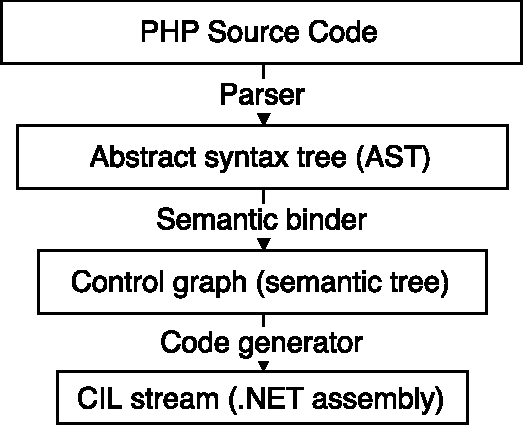
\includegraphics[scale=0.75]{../img/3_1_Peachpie}	
	\caption{Peachpie architecture.}
	\label{fig3.1:PchpComp}
\end{figure}

There is, of course, more to the compiler part. It also includes a number of code analyzers to catch common PHP bugs, provides an extensive API surface to support projects such as PHP snippets or a Visual Studio Code extension, and much more.

\section{Semantic graph}

Since our approach to implementing a generators support is based on a semantic graph transformation, let us explore it a bit more. Unlike the AST, which is a structured representation of the source code, the semantic graph corresponds more closely to an abstraction of the final program.

It knows the types of all expressions, has all method calls as well as variable/field accesses resolved and bound to specific semantic symbols, and generally contains all the information needed for a future compilation.

\subsection{Statements and expressions}

Before going into specific details about the semantic graph itself, let us properly define the difference between expressions and statements first. An expression is a combination of values and operations that produces a new value while potentially also having side effects. 

For example, plus is a binary expression that creates a new value from its two children expressions. Method call, if the method returns some value, is an expression as well. Statement, on the other hand, is an operation that only has some side effects and does not carry a value itself. A good example of a statement is goto jump.

This means that in expression trees (\autoref{fig3.3:ExpTree}), a computation abstraction where each node is an operation that takes the values of its children and produces a new value, statements can only be at the top. Since they do not have a value of their own that could be consumed by their potential parent, they simply cannot have a parent node. 

It is also good to note that while it is simple to transform an expression into a statement from - you simply throw away its value, you cannot do it the other way and use a statement in places where an expression is expected. 

\subsection{Graph structure}

With that out of the way, the semantic graph is fundamentally a forest in which every method declared in the source code or synthesized by the compiler corresponds to its control flow graph. Each graph consists of two types of elements: edges, representing control flow constructs such as loops, branches, and exception handling constructs, and blocks, simple containers holding standalone semantic statements like method calls, assignments, variable declarations, and so on. 

These individual statements, can be in the form of rather complex graphs themselves (\autoref{fig3.3:ExpTree}). They can be arbitrary expression trees with a statement at the top. For example, an assignment statement has two expression children, the variable and the one representing the value being assigned. The value expression can also be arbitrary and have children of its own and so on. Semantic expressions and statements are called bound within Peachpie.

\begin{figure}[h]
	\centering	
	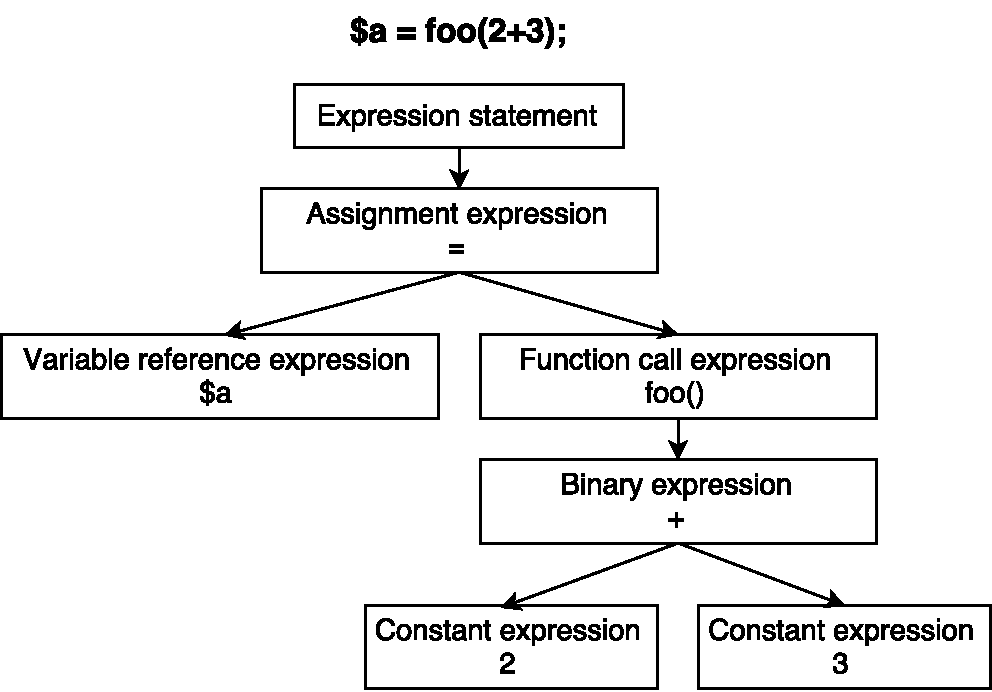
\includegraphics[scale=0.75]{../img/3_3_exprstatements}	
	\caption{Expression tree.}
	\label{fig3.3:ExpTree}
\end{figure}

The control flow edges do not have to be simple and connect only two blocks either. In fact most edges connect multiple blocks and some even have references to individual expressions (\autoref{fig3.3:Edges}). For example, a switch edge connects a source block, a switch variable expression, an arbitrary number of case blocks with their case value expressions, and an end block. Other edges are implemented similarly.

\begin{figure}[h]
	\centering	
	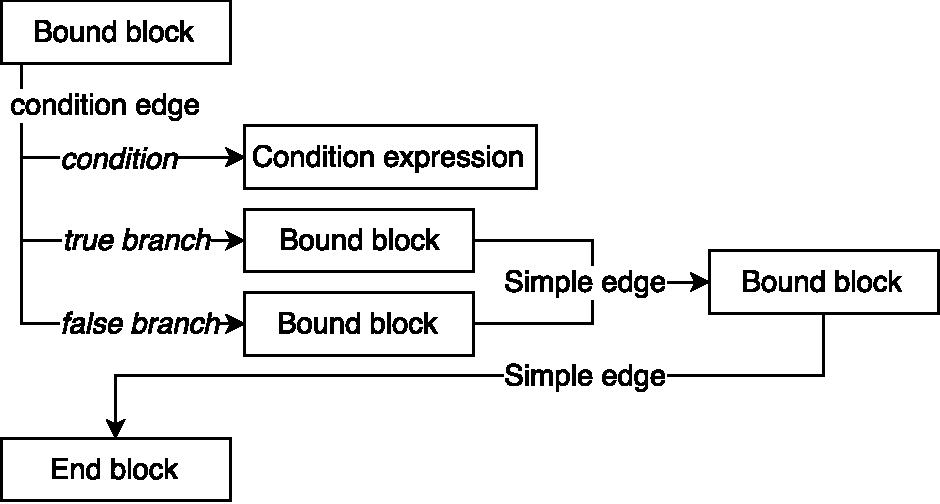
\includegraphics[scale=0.75]{../img/3_3_blocksedges}	
	\caption{Condition edge.}
	\label{fig3.3:Edges}
\end{figure}

The last type of objects to note with regards to the semantic graph are symbols. They represent declared objects. These include types, namespaces, methods, fields, variables, and parameters. Read and write accesses to fields, variables, and parameters inside methods are still represented as bound expressions, however. They are bound expressions that hold a reference to these symbols and use them as an identifier of the actual place where their value is.

\subsection{Graph creation}

There are two components in Peachpie compiler responsible for the individual method’s control flow graph creation: \emph{BuilderVisitor} and \emph{SemanticBinder}. \emph{BuilderVisitor} is a higher level component traversing the top level of a method’s abstract syntax tree and creating the aforementioned control flow edges and bound blocks in the process. 

It uses the \emph{SemanticBinder} to fill these bound blocks with bound statements and to create sporadic bound expressions needed for the edges, e.g. a switch value expression for a switch edge. Specifically, it goes through statements and control flow construct in the method’s AST and does two things. It either adds a newly bound statement into the current bound block or, on control flow constructs, creates new bound blocks. When doing so, it fills them with statements, connects them to the previous current block, and sets the last of them as the new current block.

The \emph{SemanticBinder} is a component that takes a statement or an expression in the form of an abstract syntax tree and creates its semantic representation, either a bound statement or a bound expression, that can be used in the resulting semantic graph. 

It also handles the full complexity of the statements/expressions. When it gets asked by the \emph{BuilderVisitor} to bind an assignment, it creates not only the bound assignment statement itself, but it binds its children, and their children, and so on as well, returning the full bound subgraph. 

That is the reason why the \emph{BuilderVisitor} only goes through top level statements and does not care about individual expressions. With the exception of those within edges, as noted, each expression is part of a larger expression tree under some statement that gets bind as a whole tree by the \emph{SemanticBinder}. 

\section{CIL emit phase}

In Peachpie, the CIL code generation is based solely on the semantic graph. Each of its elements, be it an edge, a statement, or a symbol, has a method, \emph{Generate} or \emph{Emit}, that can create the element’s complete CIL code representation. These methods do not produce the bytecode themselves. Instead, they use a component called \emph{CodeGenerator}, a thin wrapper around Roslyn’s \emph{ILBuilder}.


\subsection{Code generator}\label{CodeGen}
\emph{CodeGenerator} is fundamentally an abstraction of a CIL code stream. It can do two things: append either individual CIL instructions or their short sequences to the current code stream and realize the stream into actual bytecode. The only higher level service it provides is the ability to change where it should look for certain important items.

One can, for example, set an arbitrary variable as a method's \emph{this} object or specify that local variables should live in some PHP array instead of on the evaluation stack. Appending a load from a local variable then results in the correct CIL sequence being emitted. That means either a load from the locals part of the evaluation stack or, when the place of locals was changed on the current \emph{CodeGenerator}, some \emph{PhpArray}, which itself might need to get loaded from some field first. 

This is used, among other places, when there are indirect variable accesses in a method\footnote{\href{http://php.net/manual/en/language.variables.variable.php}{php.net/manual/en/language.variables.variable.php}}. Because of their indirect and thus dynamic nature, it is impossible to resolve and bind them at compilation time. In addition, there are no CIL instructions to create a new local variable nor to access a variable by its name. Afterall, local variables in CIL are just slots in the evaluation stack. Therefore, for methods with indirect variables, its locals must be moved from the evaluation stack to a \emph{PhpArray} that supports both of these operations.

\subsection{Emit}

The act of emit is very similar to the binding phase. When \emph{Generate} is called on a semantic item, it emits CIL representation of not only the item itself but also of all that is under it in the semantic graph. A code generation for a method symbol (\autoref{fig3.4:EmitOrder}), for example, causes an emit of all of its bound blocks and edges, each of which triggers the emit of their bound expressions and statements, effectively ending up generating CIL for the whole method’s body. 

As such, the emit is effectively a mixture of pre and post-order traversal of the semantic tree. First, the emit of the current item starts, subsequently its children from left to right get fully emitted, and then it finishes. Due to that and the fact that execution follows the emitted CIL code, there is an invariant. The left children represent code that is executed before the right children and nodes lower in the tree finish before their parents. 

\begin{figure}[h]
	\centering	
	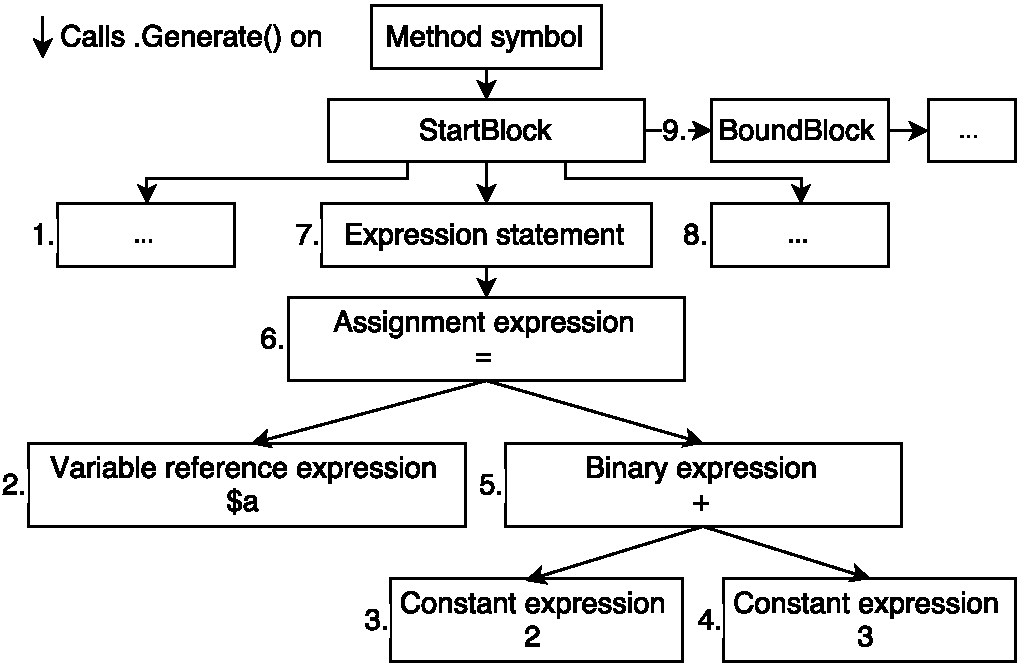
\includegraphics[scale=0.75]{../img/3_4_emitorder}	
	\caption{Emit order of a method.}
	\label{fig3.4:EmitOrder}
\end{figure}

The individual \emph{Generate} or \emph{Emit} methods are completely independent. They only append CIL instructions representing their semantic node to the \emph{CodeGenerator} instance they got passed as a parameter. In case their respective nodes have any children within the semantic graph, they also call \emph{Generate} on them, always passing the \emph{CodeGenerator} instance they themselves got. This ensures that in the end, the one \emph{CodeGenerator} instance contains CIL code for all the method’s statements, expressions, and edges.


\subsection{Generate methods’ invariants}

While individual nodes can emit themselves however they want, there are two rules that must hold true. The code emitted by a bound expression must load and leave its value on the top of the evaluation stack. Other than that, it cannot leave anything else there nor can it remove something. Their \emph{Generate} methods also have to return a symbol representing the expression’s IL type. 

For bound blocks, statements, and edges, the rule is similar with the difference that, since they do not have an inherent value, they cannot leave anything on the evaluation stack at all. Their methods do not return anything.

These rules ensure a number of things. First, all expressions are basically interchangeable. An emit of a binary expression does not need to care about the operands’ types. It can simply call \emph{Generate} on them and know that the evaluation stack will contain their values, independent on whether they are constant expressions, method calls, or something else.

Also, since neither statements nor edges can leave anything on the evaluation stack and statements can only be at the top level of the semantic tree, the evaluation stack is guaranteed to be empty in the beginning of each bound statement’s execution. This is important because there are statements, such as return or goto, that transfer execution and therefore need the evaluation stack to be empty.

\section{Peachpie runtime library}

The runtime library consists of a number of important types needed to support the dynamic nature of PHP. Probably the most important one is \emph{PhpValue}, a managed counterpart of the Zend Engine’s \emph{ZVal}\footnote{\href{http://php.net/manual/en/internals2.variables.intro.php}{php.net/manual/en/internals2.variables.intro.php}}. It is a type used everywhere the data-flow analysis can not ensure a more specific type. It is a lightweight structure that can hold a primitive value (number, string, or boolean), \emph{PhpArray} (essentially a hashtable), reference to a proper class instance, or - in case of a reference variable - a link to another \emph{PhpValue}. It also supports all the required type conversions and serves as a true representation for an arbitrary PHP value.

Another core type present in the runtime library is \emph{Context}. As suggested by its name, it holds the context of the current execution. It contains defined global methods, variables, and constants, the value of static fields, and much more. It is a rather special type because it gets silently passed to every PHP method as their first argument throughout the whole execution.

When a library originally written in PHP is used from another .NET language (C\#, F\#, …), the context has to be explicitly created and passed into it as part of the method's invocation. If the original PHP app is used on its own, the context gets created automatically in the beginning before any user code is run.

Other than that, the runtime library also contains a function call and variable access resolution logic needed to support dynamic behaviors at runtime, a variety of types needed for certain PHP features, such as base class for lambdas, and a full reflection support. 

\chapter{Generators in other platforms}

In this chapter we will take look at two very different approaches towards supporting generators. First we will describe the way they are implemented by C\# compiler Roslyn. The combination of Roslyn and C\# was chosen because despite the differences between generators in C\# and PHP it is still very similar to our Peachpie and PHP mix.

Both Roslyn and Peachpie compile their respective languages into CIL, Peachpie’s compiler is de facto based on Roslyn’s architecture, and generators in PHP are fundamentally a superset of what they are in C\#. 

IronPython and its compiler based on DLR was also considered, mainly due to python’s generators being closer to PHP’s. Similarity of compiler platforms and the fact that IronPython offloads a lot of details to DLR, which is by design generic and therefore needlessly complicated for our use, prevailed, however. 

The second implementation we will talk about in this chapter is Zend Engine’s for PHP generators. In spite of the fact that we cannot use it as an inspiration because it relies on native support by runtime it is useful to mention it at least briefly. It is the implementation we are trying to mimic, afterall.

\section{CSharp and Roslyn}\label{sec:3:1}

As said previously CIL, into which .NET implementation of C\# gets compiled, does not have a native understanding of generators. There is, for example, no instruction to yield or to automatically construct an iterator type instance with all the appropriate methods. Therefore the Roslyn compiler has to support generators by lowering them, in essence transforming them into lower level language constructs. 

There are two main components responsible for that. First, there is a rewriter that takes the original generator method and transforms it into a normal method that only uses constructs CIL supports. For example it rewrites all the yield statements. We will come back to it later. Then there is a type implementing the \emph{IEnumerator} interface (\autoref{fig1.1:iterators}) whose instance gets returned from the generator method and which actually represents the generator.


\subsection{Iterator object and generator methods}

There is no single type implementing the \emph{IEnumerator} interface. For each generator method the Roslyn compiler synthesizes one separate iterator type. While most of their \emph{IEnumerator} methods are simple and actually the same for all of them there is one that is always unique, the \emph{next} method. This one actually contains the implementation of the original generator method only now transformed and turned into a state machine by the rewriter.

The actual original generator method has its body replaced with compiler generated code that instantiates, initiates, and returns the corresponding synthesized type (\autoref{fig4.1:GenMethod}). Therefore it is a normal CIL method that returns an iterator. An iterator containing a transformed version of the method’s original body as its \emph{next} method.

\begin{figure}[h]
	\centering	
	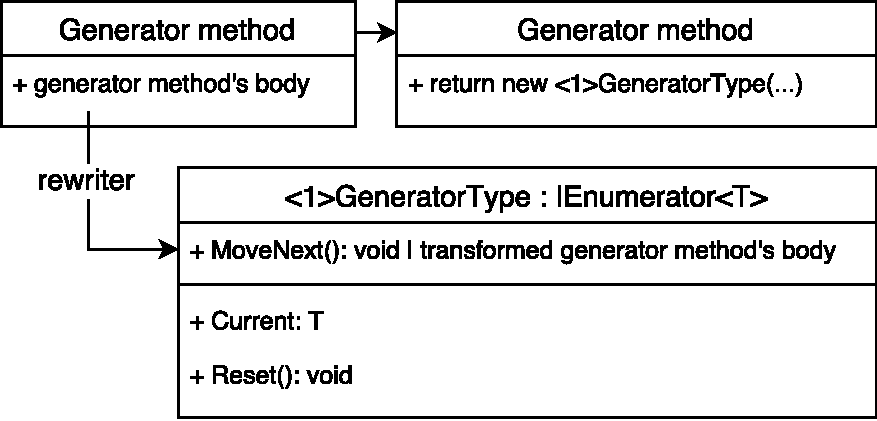
\includegraphics[scale=0.75]{../img/4_1_generatormethods}	
	\caption{Generator method, generator's next method, and the generator type.}
	\label{fig4.1:GenMethod}
\end{figure}

\subsection{Rewriter}

The rewriter has to take care of three things while transforming the original generator method’s body into the iterator’s \emph{next} method. It has to handle fixing references that expected the method to be where it was instead of on the generated type, state saving on yields, and state retrieval in the beginning. 

The only references that care where the method actually is are references to \emph{this}. Fortunately, \emph{this} instance can simply be captured in the original generator method, passed to the generator during its initialization phase, and kept there in a field. All references to the original \emph{this} variable can then be rewritten to references to a generator’s field holding the captured \emph{this} instance.

As of state saving, due to the fact that yield is only a statement in C\# and an invariant in Roslyn, that the evaluation stack is always empty in between separate statements, there are guaranteed to be no temporal values on the stack before yields get executed. This means that the only state that needs to be saved are local variables, parameters, and the position, in essence the next statement to be executed.


\subsection{Local variables parameters}

To handle the first two thirds of the state, the rewriter creates a new field on the corresponding iterator type for each local variable and parameter. Then it replaces all, both read and write, references to these original local variables and parameters with references to the newly created fields (\autoref{fig4.1:LocVars}). The result is that there are no accesses to local variables or parameters in the rewritten method. Also all values now live on the iterator instance which means they are persistent in between individual calls to the \emph{next} method.

The situation regarding parameters is, in fact, a bit more complicated. As defined by the \emph{IEnumerator} interface the \emph{next} method cannot have any parameters. Fortunately, there are no references to parameters inside the \emph{next} method after the rewrite, only to the instance fields they got replaced with. The fields still need to be initialized with their values, however.

That can be done similarly as the this reference was handled in the original generator method. The method has access to both the original parameters and the iterator instance before any code from the \emph{next} method has any chance to access the fields. Hence, after the iterator instance is created, the parameter values get assigned to their corresponding fields as part of an iterator’s initialization phase.

\begin{figure}[h]
	\centering	
	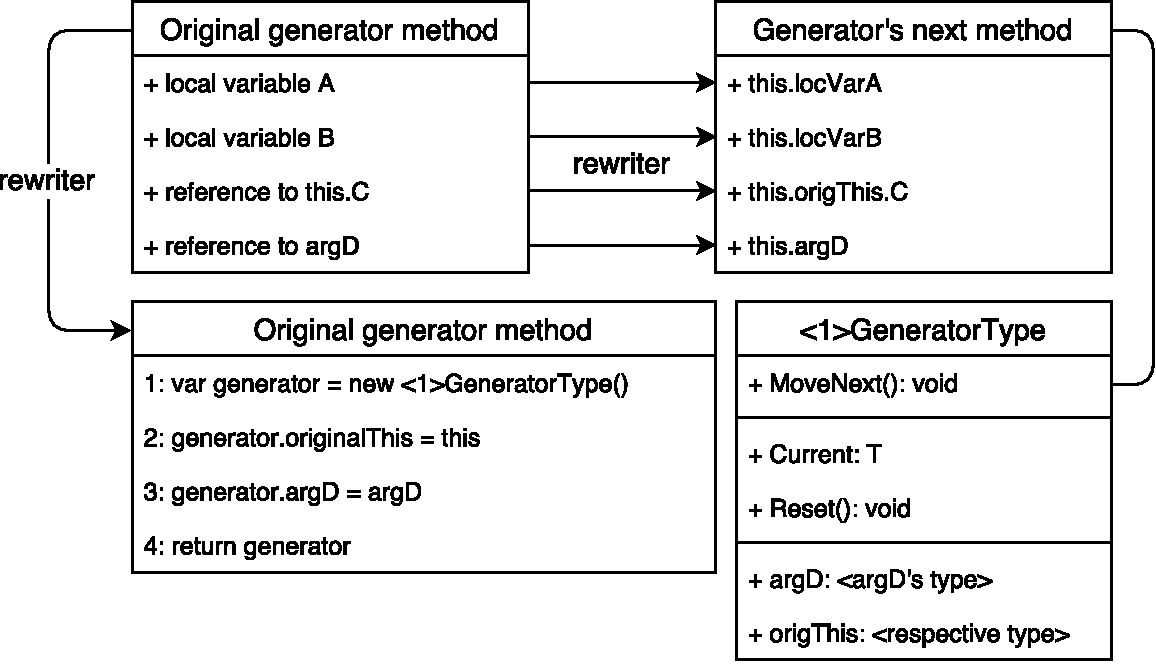
\includegraphics[scale=0.70]{../img/4_1_localVars}	
	\caption{Local variables rewrite for generator methods.}
	\label{fig4.1:LocVars}
\end{figure}

\subsection{Execution position}

The last thing that needs to be taken care of is saving the point where the last yield happened, effectively the place a subsequent call of the \emph{next} method should continue from. To handle that the rewriter does two main things. It replaces each \emph{yield} with a number of statements and creates a jump table in the beginning of the \emph{next} method (\autoref{fig4.1:Position}). A new field called state, representing which yield the generator exited with last time, is also created on the iterator instance.

Each \emph{yield} gets lowered into four separate statements. First, an assignment of the yielded value to a current field on the iterator instance. This field is used by the \emph{IEnumerator}'s \emph{current} method as its backing field. Second, an assignment of the current \emph{yield}’s index to a state field on the iterator instance. The order of these indexes can be arbitrary, only uniqueness among other \emph{yield}’s indexes within the same method is required. Third, a normal return from the \emph{next} method. And finally, a \emph{yield}’s label based on its index that can be used as a target for jumps.

The jump table in the beginning of the \emph{next} method is fundamentally a switch statement that, based on the current value of the iterator’s state field, jumps to a corresponding \emph{yield}'s label. Within the four statements created by rewriting one yield the state field assignment and the label are connected. The assignment sets a state value whose corresponding case in the switch table contains a jump to the label. And since the indexes and therefore states are unique it is guaranteed that this always holds true.

\begin{figure}[h]
	\centering	
	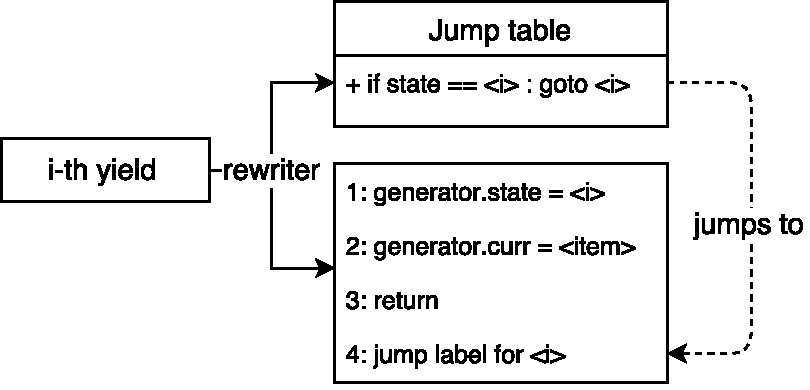
\includegraphics[scale=0.75]{../img/4_1_position}	
	\caption{Local variables rewrite for generator methods.}
	\label{fig4.1:Position}
\end{figure}

That way when the \emph{next} method is called repeatedly it always resumes with the statement that is directly after the return the method exited with before. This happens simply due to the fact that whenever you hit a \emph{yield}, and therefore a return, two things are true. 

First, just before returning from the \emph{next} method an index of the hit \emph{text} gets assigned to the state field. Second, the state field does not change unless the \emph{next} method is called again. And when that happens, the switch table in the beginning of the \emph{next} method jumps to the label that was created by rewriting the same \emph{yield} as the last evaluated state assignment. Which is, as we have already proven, the label directly after the return the method exited with previously.

\begin{listing}[H]
\caption{Original and rewritten generator method's body.}
\label{list4.1:generatorRewrite}
\begin{minted}{csharp}
// Original method's body
Yield 5;
Yield 10;

// New method's body
switch(this.state){
  case 1:
    goto: Label_1;
    break;
  case 2:
    goto: Label_2;
    break;
}

this.current = 5;
this.state = 1;
return;
Label_1;

this.current = 10;
this.state = 2;
return;
Label_2;
\end{minted}
\end{listing}

Naturally, this is not all the Roslyn compiler does to support generators in C\#. It is, however, more than enough for us to design our own implementation in the Peachpie compiler. 


\section{PHP and Zend Engine}

Unlike CIL and CLR respectively, the reference PHP runtime Zend Engine understands generators natively \citep{ZendGen}. As such it is able to execute yields without having to lower them into simpler PHP constructs.

Not going into details and slightly simplifying, the execution state of Zend engine is represented by a virtual machine stack. This stack contains individual stack frames, each corresponding to a method’s execution. When a method is called a new stack frame gets created, initiated, and pushed on top of the stack. When it returns its stack frame gets popped.

Each frame contains the complete information about a method’s execution state, such as all local and temporal variables, arguments, returned value, and an index of the last executed statement, to name a few. Therefore if one needed to save the execution state of a method storing its frame stack would be enough.

And that is exactly what the Zend engine does when it encounters a yield expression. It creates a new generator object, copies the current stack frame into it, does some other things like sets its current key and value, and returns it. In this context the current stack frame is the one representing the execution state of the method with yields therefore, in essence the generator method.

Later, when the \emph{next} method is called on the generator instance, it restores a stack frame previously saved on the generator object to the top of the virtual machine stack and resumes execution. This effectively causes the generator method’s execution to continue from the very point where the last yield was encountered and thus where it stopped. On subsequent yields the runtime sets the generator’s fields such as key and current, updates its saved stack frame representing the generator’s method current state, and returns.

The description above is obviously a simplification of the actual process that happens in the Zend engine with details regarding yields in exception blocks and inside function calls completely omitted. However, it still provides a good high level overview of how generators are implemented in PHP’s reference runtime and how it is different to Roslyn’s approach.  

\chapter{Generators in Peachpie}

The goal of this thesis is to enable Peachpie compiler to handle PHP generator methods while keeping as much of their original semantics as possible. That means we do not want to change their behavior and want to enable all the features they offer in PHP, only now compiled to CIL and executed either by the CLR or another CLI environment.
 
As noted in previous chapters\footnote{Chapter \ref{sec:3:1}}, this in itself is complicated, because unlike the PHP runtime Zend Engine, the CIL and CLR do not have a native support for generators or generally pausing the execution of a method at arbitrary points. Also, almost all other CIL based languages with generators, such as C\# or F\#, that implement them by compiler transformations have them in a substantially more limited form than PHP.

Other than that, we also want to reuse existing Peachpie infrastructure and only implement generator specific bits when necessary. While this goal is not as important for our immediate work, it is necessary for the project as a whole. Cluttering the compiler with logic for a feature that is not actually used as often would simply be inexcusable.

\section{Basic generators implementation}

Before dealing with all the complexities of PHP’s generators, let us first explore how an implementation of their limited subset would work within Peachpie. Specifically, we will ignore \emph{yield} in exception handling blocks and expect it to be only in places where it could happen as a statement, i.e. no \emph{yield} inside an expression tree, for this chapter. 

Much like Roslyn’s approach, our implementation of generators within Peachpie will also be based on transforming the original generator method into an iterator's \emph{next} method. So as not to repeat ourselves, we will only point out the differences in the next section.

\subsection{Iterator object}

Unlike in C\#, where generator methods are free to return any object implementing an \emph{IEnumerator} interface, the PHP specification dictates that the returned object must be an instance of a \emph{Generator} type \citep{GenPHP, GenPHPRFC}. This means that in Peachpie we cannot just synthesize a new type for each generator method as Roslyn does.

If we were to do that, all reflection methods and type checks would report the actual synthesized type on the returned iterator instance instead of the \emph{Generator} type, as required by PHP’s specification . We could theoretically hard code exceptions for these synthesized types into all methods that query an instance’s type, but that would go against our goal to implement as little feature specific code as possible.

Instead, we must create one generator type in Peachpie’s runtime library and use it as a basis for all generator methods to return. That approach, however, carries some limitations with it. The generator type can now include only shared code and fields. That means neither a specific \emph{next} method’s implementation nor fields for lifted local variables from said method.

Other than that, the \emph{Generator} type can be practically the same as the ones synthesized by Roslyn as it is a simple implementation of PHP's \emph{Iterator} interface (\autoref{list5.1:GeneratorType}). It can hold a captured reference to the \emph{this} instance of the original generator method, a state field to know what point the \emph{next} method should continue from,  fields for the \emph{current} element and, since we are in PHP now, its \emph{key}.

\begin{listing}[H]
\caption{Simplified version of the Generator type.}
\label{list5.1:GeneratorType}
\begin{minted}{csharp}
public delegate void GeneratorStateMachineDelegate(
  Context ctx, object @this, PhpArray locals, 
  Generator gen);
public class Generator : Iterator
{
  readonly Context _ctx;
  readonly GeneratorStateMachineDelegate _stateMachineMethod;
  readonly object _this;
  readonly PhpArray _locals;
  internal int _state = 0;
  internal PhpValue _currValue, _currKey;
  public void next() =>
  _stateMachineMethod.Invoke(_ctx, _this, _locals, gen: this);
}
\end{minted}
\end{listing}

\subsection{Next method implementation and local variables}

The \emph{next} method's implementation problem is easily solvable. The shared generator type can hold a delegate to an implementation of the \emph{next} method instead of the method itself. This enables Peachpie compiler to synthesize the \emph{next} method anywhere and then to assign its delegate to the generator. The generator must still implement some \emph{next} method to comply with the Iterator interface but it can be a shim that only calls the saved delegate.

There is only one restriction with regards to the actual \emph{next} method’s placement. The transformed method must be accessible from within the original generator method. The reason is that the original method is where the instantiation and initialization of the generator, thus also the creation and assigning of the delegate, happens. 

One such suitable place is the enclosing type of the original method, where it can always be synthesized as a static method. It being a static method is not a problem because, as mentioned in the chapter about Roslyn’s implementation, a reference to the enclosing type’s instance is passed as a \emph{this} parameter. And since the enclosing type could be a static class, it cannot be a normal instance method anyway.

The inability to add fields to the generator type can also be overcome. As described in the CIL emit phase chapter\footnote{Chapter \ref{CodeGen}}, Peachie's \emph{CodeGenerator} supports specifying where local variables should live within a method with the option to, for example, move them to a \emph{PhpArray}.

With that, a \emph{PhpArray} field can be added to the generator type and we can specify that all of the \emph{next} method's local variables should live on it. Because parameters are considered local variables in Peachpie, this approach handles them as well. They only need to be initialized with their values in the original generator method. That way, the \emph{next} method’s local variables and parameters get lifted to the generator type the same way as in Roslyn, with the only difference being that they do not get lifted to individual fields but to a single \emph{PhpArray} (\autoref{fig5.1:Generator}).

\subsection{Accessibility of fields on the Generator type}

Moving the \emph{next} method outside of the generator type means that the method cannot access its fields such as \emph{current} or state directly through a \emph{this} reference. That is a problem, because the method needs to both read and write these fields to progress the generator. An effective solution is to pass the generator instance as a parameter through the \emph{next} method delegate - in essence to not only call the delegate from within the generator’s own \emph{next} method, but to call it with a \emph{this} reference as a parameter.

That on its own would be enough if all the fields on the generator type were public. That is, however, not our objective. We want the generator type to have the same public API as it does in PHP and there are no such public fields in PHP’s \emph{Generator}. Therefore, we need to find a way to access the fields from a method within the user’s assembly, the transformed \emph{next} method the generator has a delegate to, without having to make the fields accessible to other user code.

One way to do this is to make the generator fields internal and create public getter and setter methods for these fields in the Runtime library. Since the generator type also lives there, the methods can access its fields and, because they are public, they can be used from within the synthesized \emph{next} method (\autoref{fig5.1:Generator}). The methods can be simple static getters and setters, always taking a generator instance as a first parameter and either returning an appropriate field’s value or taking its value as a second parameter and then setting it on the instance.

\begin{figure}[h]
	\centering	
	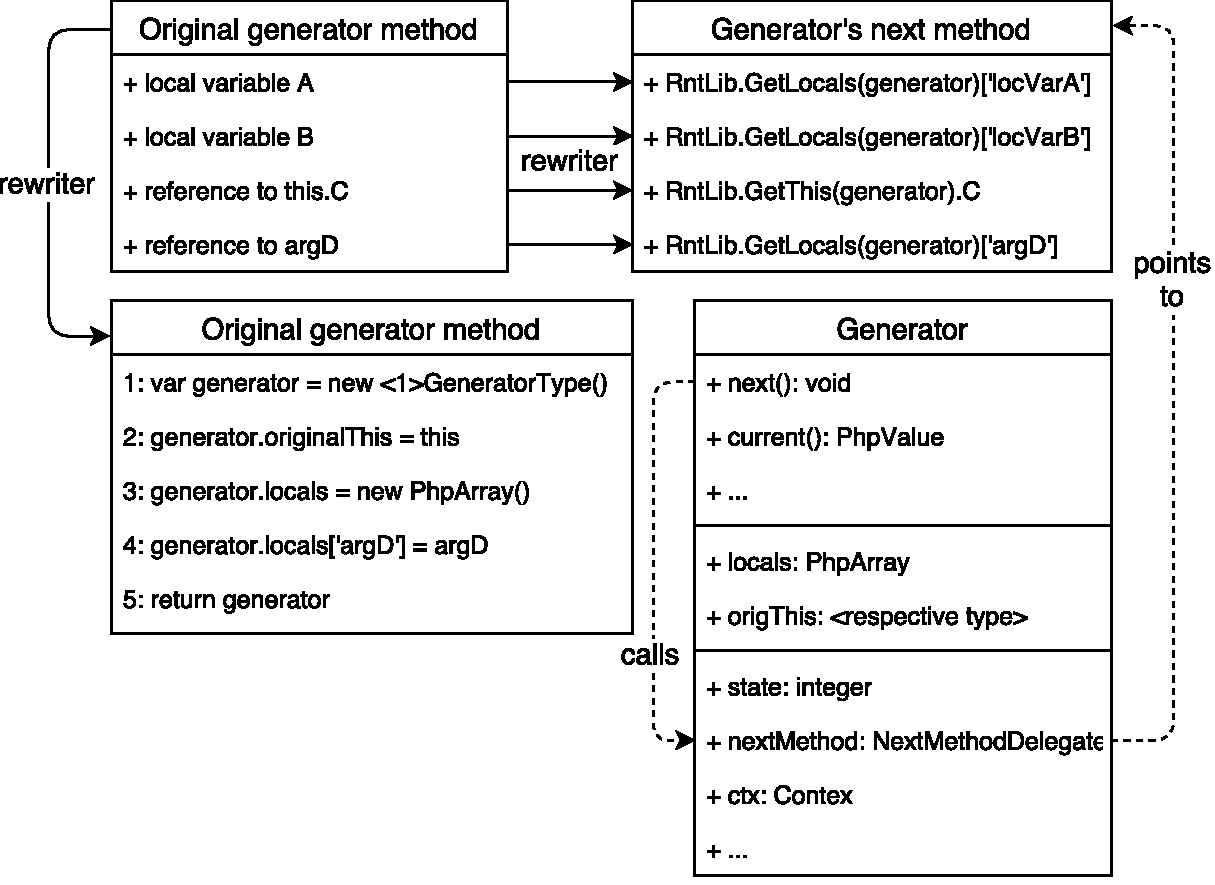
\includegraphics[scale=0.70]{../img/5_1_Generator}	
	\caption{Transformation of the generator method.}
	\label{fig5.1:Generator}
\end{figure}

While it is true that this approach still opens a way for the user to modify the generator’s internal state, it has to be done through special methods from Peachpie runtime library and as such, it can hardly be done by accident. It also ensures a compliant public API of the \emph{Generator} type.

\subsection{Context handling}

Being in PHP, we need to ensure that the correct PHP \emph{Context} gets passed to our moved \emph{next} method. There are two ways to do it. Current \emph{context} can either be passed as part of each call to the generator methods, and subsequently via a delegate to the \emph{next} method, or it can be captured once during the generator’s initialization and then reused the same way as is the \emph{this} instance.

Neither approach is inherently wrong. Passing the \emph{context} with each call ensures the current one is used even in situations where one generator instance is used with multiple PHP \emph{context}s. That can happen, for example, when PHP code is called from some other .NET language and multiple \emph{context}s are created manually. This approach is also more in line with how \emph{context} on normal instances is handled. It is not captured in the constructor and then used by all the instance methods, but always passed as a parameter.

On the other hand, capturing the \emph{context} on the generator’s creation better represents the idea that the generator is a fully self-contained object. It is also marginally easier to implement and provides better opportunities for interop between PHP generators and other .NET languages. This way, a generator can be created in PHP and then used elsewhere as a normal iterator, without having to explicitly keep and supply its \emph{context}. Thus, the capture once in the original generator method approach was chosen.

\subsection{Rewriter}

Due to architectural differences, we will not have a standalone rewriter component in Peachpie. While it would be possible, there are, as of writing this thesis, no other candidates that could make use of them within the compiler. And adding a generic support just to have one rewriter for generators goes against our goal to keep the implementation as simple as possible. Instead, our implementation will rely on support by the \emph{SemanticBinder}, slightly changed emit of a \emph{MethodSymbol} and \emph{StartBlock}\footnote{Chapter \ref{StartBlock}}, and a new semantic node. 

As long as we limit ourselves to \emph{yield} only at places where it could be as a statement, which is the temporal restriction we have set for this chapter, the support provided by the \emph{SemanticBinder} can be minimal. It needs to do two things: bind the new semantic object - \emph{BoundYieldExpression} - when it encounters the AST’s \emph{YieldExpression} and mark the method’s symbol as a generator. 

\subsection{Bound yield expression}

The \emph{BoundYieldExpression} can be a rather simple semantic node with two children: the yielded key and yielded value expressions. It should generate CIL to set the yielded key and value fields on the generator instance, update its state, \emph{return}, and mark a label for the subsequent continuation (\autoref{fig5.1:Rewriter}). 

Due to being an expression, albeit for this chapter limited to places where it could also be a statement, it needs to push and leave its value on the evaluation stack. However, since its value will not be needed due to our restriction, it can just as well be an empty \emph{PhpValue}. The value will always get discarded, anyway. The restriction also handles the problem that we are emitting a \emph{return} from within an expression, i.e. in a situation in which the evaluation stack might not be empty.

It is true that all of the \emph{BoundYieldExpression} could be replaced with a number of normal PHP statements by lowering. That would, however, require the \emph{SemanticBinder} to be able to produce multiple semantic statements for only one AST node, and for the \emph{BuilderVisitor} to accept them. And while such support could be added, it was decided that it would be too complex.

\begin{figure}[h]
	\centering	
	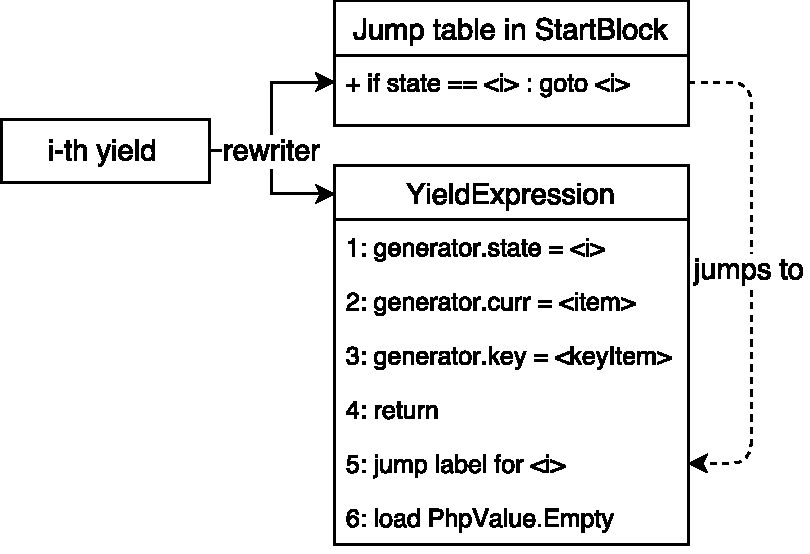
\includegraphics[scale=0.75]{../img/5_1_rewriter}	
	\caption{Rewrite of a yield expression.}
	\label{fig5.1:Rewriter}
\end{figure}


\subsection{Start block}\label{StartBlock}

The \emph{StartBlock} is a special instance of a \emph{BoundBlock} that is present in the beginning of each method’s control flow graph (\autoref{fig3.4:EmitOrder}). As such, its emit routine is the perfect place to generate a jump table for generator methods. It can, when its enclosing method symbol is a generator, query all present \emph{yield} statements that were previously set by, for example, the semantic binder and generate the whole jump table.

\subsection{Method symbol}\label{MethdSymbol}

The method symbol’s emit must be changed as well. When it represents a generator, it cannot simply generate the CIL representation of its body. If it did that, it would not produce a method that returns an iterator as it should, but a method that implements the iterator’s \emph{next} method.

Instead, three things need to happen. First, a new static method representing the generator’s \emph{next} method must be synthesized in the enclosing type. Second, the original body needs to be emitted inside the synthesized method with its \emph{CodeGenerator} set to offload local variables into a generator’s locals field. As explained earlier, the synthesized \emph{next} method accepts a \emph{Generator} as a parameter.

Third, a sequence of statements that create, initiate, and \emph{return} a \emph{Generator} instance must be emitted as the actual current method symbol’s body, producing a method that returns an iterator. As part of the initiation phase a delegate to the synthesized \emph{next} method must get created and assigned to the newly constructed generator instance. Also, values of all parameters need to get copied to the generator’s locals array, as previously discussed.

\section{Yield as an expression - theory}\label{AlghTheory}

With that, we have described a design of a generator’s compilation within the Peachpie platform with a featureset limited to more or less C\# generators. Now, let us broaden it with the support for \emph{yield} as an expression. Before going into details on the specific implementation, let us first take a look at the general idea behind our approach. 

As said before, a \emph{yield} being an expression is a problem, because an expression can happen in a situation where the CIL evaluation stack might not be empty. Since \emph{yield}s include a \emph{return} and returning with a non-empty evaluation stack is forbidden, it does not go well together. Even if it were allowed, there would still be the problem that the non-empty evaluation stack would represent some sort of state - one that would need to get saved and then retrieved upon the continuation.

\subsection{Possible approaches}

Fundamentally, there are two possible ways to approach this problem. One can either come up with a mechanism to save and then retrieve the evaluation stack or rearrange the semantic graph so that \emph{yield}s are only in places where they could happen as statements.

While the first approach might be appealing, after all it more closely mimics the Zend Engine’s way of handling yields\footnote{Chapter \ref{ZendGen}}, it is almost impossible to implement. Because the CIL does not have any instructions to query the contents or to completely save/load the evaluation stack, the compiler would have to do it manually. That means it would have to track the stack’s content throughout the compilation and then emit individual instructions to save/load its content, one element at a time.

That would mean two things. First, we would either have to create our own version of the \emph{CodeGenerator} that would be able to keep track of what the evaluation stack contains at any moment or we would have to change the emit of each semantic node to save the information about what it puts on the stack explicitly. Both of these would be relatively complex to do and, in case of the second approach, even to maintain due to possible new semantic nodes. Second, either of them would mean an increase in memory usage because we would need to remember information previously not required, all of which just to support only a \emph{yield} as an expression. 

On the other hand, the second approach, to rearrange the semantic tree, requires only a few local implementation changes and does not cause a substantial memory consumption increase. Essentially, it is based on the idea that we can break an expression tree into a series of statements while keeping the meaning and order of execution the same.

\subsection{Branch capture \& yield splitting}\label{Capture}

There are two important observations required for this method. First, a \emph{yield} can be broken into two semantic nodes. A statement that does the value and key setting, state saving, \emph{return}, and marking the continuation label, acting as the equivalent of a C\# \emph{yield} statement. The other node is an expression that represents the sent value. If the expression directly follows the statement, the result is, in terms of emitted CIL, the same as with one combined \emph{yield expression} (\autoref{fig5.2:Splitting}). 


\begin{figure}[h]
	\centering	
	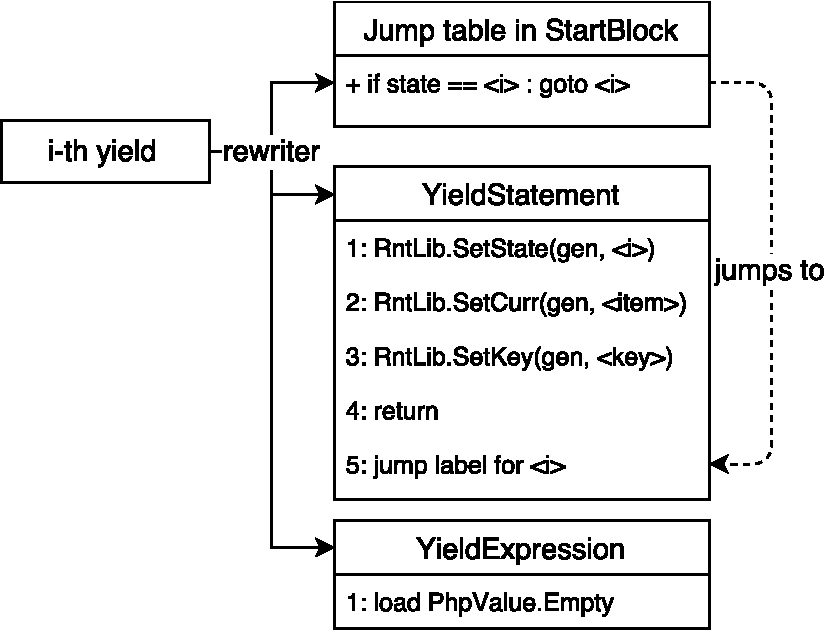
\includegraphics[scale=0.75]{../img/5_2_yieldSplitting}	
	\caption{Splitting of a yield into an expression and a statement.}
	\label{fig5.2:Splitting}
\end{figure}

Second, we can cut any branch in an expression tree and prepend it before the tree while keeping the meaning of the program the same except for the order of execution. To do it, we need to create a temporal variable, replace the branch in the tree with a read from said variable, and prepend the tree with a statement that assigns the branch that was replaced to the variable it was replaced with (\autoref{fig5.2:CaptureBranch}). Let us call this process capturing a branch.

The problem with the order of execution is that the captured branch, being lifted to the prepended statement, will get executed before any other expression from the tree. Even before all the expressions in branches that might be to the left of the captured branch and that were therefore supposed to be executed first. In the figure below, the expressions $5$ and $6$ respectively will get executed first, even though they should come after expressions $1$, $2$, $3$, and $4$.


\begin{figure}[h]
	\centering	
	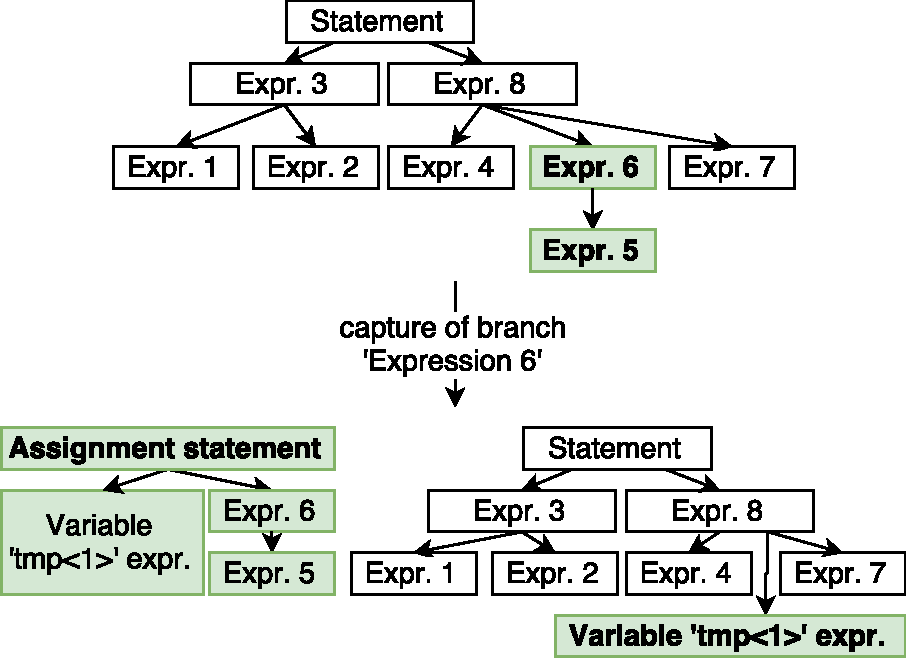
\includegraphics[scale=0.75]{../img/5_2_capturing}	
	\caption{Capturing a sole branch.}
	\label{fig5.2:CaptureBranch}
\end{figure}

An obvious solution to this problem is to cut and prepend not only the one branch we want to capture, but also, in their respective order from left to right, all other branches that are supposed to get executed before it (\autoref{fig5.2:CaptureAllBranch}). Since the semantic graph emit, and thus also the execution, follows a post-order traversal, we must cut and prepend all branches that are higher and to the left of the branch we want to capture. 

To be specific, that includes all branches that start to the left of the path between the root of our captured branch and the root of the whole semantic graph. The reason lies in a post-order traversal of the semantic graph. 

It starts with the graph’s root. Then it goes through the root’s leftmost child, followed by its next child, and so on. Let us say, for example, that the second element of our aforementioned path is the root’s third child. When the traversal enters it after going through the branches started by the root’s first two children, it goes into its leftmost child first, again. It then continues the same way until it encounters the root of our branch. When that happens, it keeps following the same logic, traversing the whole branch before closing its root and starting to visit any other nodes. After the traversal is finished with the branch, it closes its root and goes one level up, starting to traverse the branch’s root’s first sibling to the right.   

All other expressions, be it those directly on the path or on branches to the right, are supposed to be evaluated after our branch and, as such, do not have to be cut and prepended. The ones on the path have our branch among their children and thus need its result - our branch - to be evaluated first. And the ones on the right need to be evaluated later, simply because of post-order traversal rules. 

\begin{figure}[h]
	\centering	
	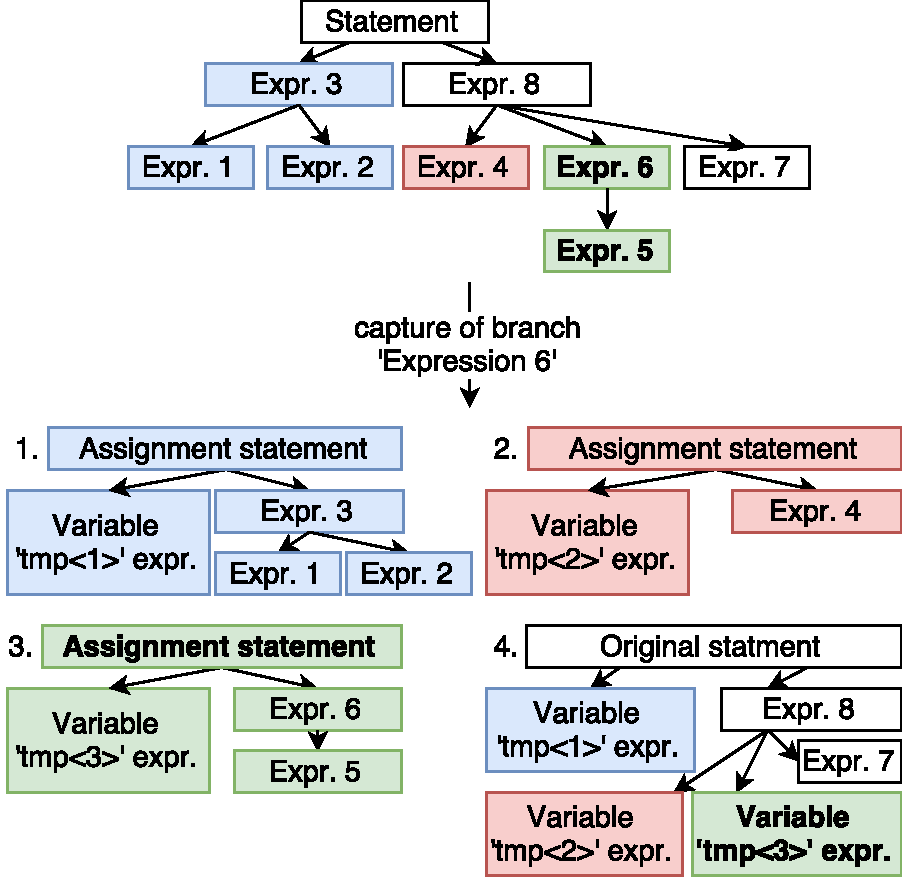
\includegraphics[scale=0.75]{../img/5_2_captureAllOnPath}	
	\caption{Capturing a whole branch while maintaining execution order.}
	\label{fig5.2:CaptureAllBranch}
\end{figure}

\subsection{Semantic tree transformation}

Now we can combine the two observations from the beginning of the previous section and come up with a solution to our \emph{yield} as an expression problem. Our goal is to split each \emph{yield} and then separate its statement part while maintaining the original order of execution.

To be able to do it, the \emph{yield} has to be on top of an expression tree first. It must be, in terms of execution order, its first user code representing node. When that is true, we can split the \emph{yield} into a \emph{yield expression} and a \emph{yield statement}, and then put the statement part before the tree. 

This does not change the program’s meaning or order of execution, because the \emph{yield statement} is directly followed by the tree and the tree’s first user code node is the \emph{yield} expression. And since the part of the \emph{yield} containing a \emph{return} is a proper statement before - not inside - a tree, the semantic graph is actually emitable.

With that, our problem has shifted to transforming expression trees containing \emph{yield}s at arbitrary places into multiple expression trees that have them only as their first user code representing nodes. If we were able to do that, we could split each of the \emph{yield}s and separate their \emph{return} containing parts as standalone statements.

The transformation can be done through our branch capturing mechanism. We can take each branch that starts with a \emph{yield} and capture it (\autoref{fig5.2:CaptureYield}). That prepends its tree with an assignment of the captured branch and all other branches that are, within the tree, supposed to get executed before it. None of the other branches are of significance for us, so let us ignore them and focus only on the captured one. 

The tree representing a prepended assignment of the capture branch contains a \emph{yield} as its first expression that is not the synthesized \emph{assignment statement} itself. This holds true, because we specifically captured a branch that starts with a \emph{yield}. As such, the tree representing the prepended branch fully adheres to our requirements for splitting the \emph{yield} into a statement and an expression.

\begin{figure}[h]
	\centering	
	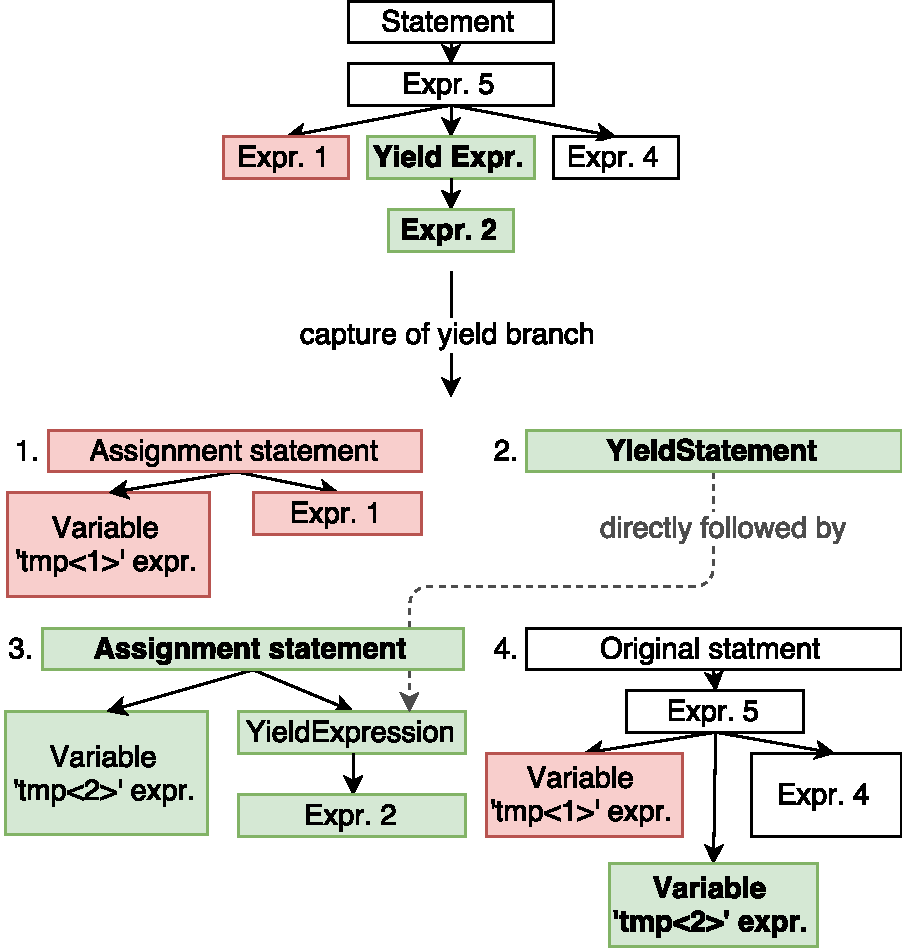
\includegraphics[scale=0.75]{../img/5_2_yieldCapturing}	
	\caption{Capturing a whole branch starting with a yield.}
	\label{fig5.2:CaptureYield}
\end{figure}

Now we have to repeat the aforementioned process for each expression tree containing \emph{yield}s and for each of their branches that starts with them. Every run of our algorithm fixes one \emph{yield} and results in a correct semantic graph that can serve as a starting point for another run. This means that after a finite number of repetitions, all \emph{yield}s will have been split while keeping the original program’s meaning and execution order intact.

\subsection{Short circuit evaluation}\label{shortCircTheory}

The solution from the previous section would work perfectly, if it were certain that all branches of an expression tree will always get evaluated. The problem is that they do not. For example, a conditional operator \emph{? :} is represented by an expression that has three children, only two of which get evaluated in any given situation. Its children are a \emph{condition expression} that gets evaluated first and every time, and two \emph{conditioned expression}s representing its return value. One that gets evaluated and returned when the condition turns out to be true and one for when it is false. A similar situation transpires with short-circuit evaluated binary expressions such as coalesce, and, and or operators.

The problem is that a \emph{yield} can be inside one of these \emph{conditioned branches} and when its gets captured and prepended before the tree, it will always get executed regardless of the \emph{condition}. For example, even if the \emph{condition} were false, an expression tree for its true branch, being prepended before the tree because it includes a \emph{yield}, would still get executed and had its result saved into a temporal variable. The variable would simply not get used as a result of the \emph{condition expression} (\autoref{list5.3:CondNotGuarded}).

\begin{listing}[H]
\caption{Conditional expression whose captured branch is not conditioned.}
\label{list5.3:CondNotGuarded}
\begin{minted}{php}
<?php
// Original expression before capturing the yield branch.
$result = isTrue() ? yield 0 : "falseBr";

// Expression with a captured yield branch.
$tmpBranch = yield 0; // The yield is evaluated everytime.
$result = isTrue() ? $tmpBranch : "falseBr";
\end{minted}
\end{listing}

This, of course, represents a problem. While the result of each expression would remain correct, a whole expression branch would now get executed every time instead of only when a certain condition was satisfied. And even if the branch itself did not have any side effects, it starts with a \emph{yield} which includes a \emph{return}. A \emph{return} that was previously conditioned but is now executed every time.

Fortunately, the solution is relatively simple. When going through the semantic graph to capture branches starting with a \emph{yield}, the mechanism can remember when it enters and leaves a \emph{conditioned branch}. And when it is about to capture a sub-branch while being in a \emph{conditioned branch}, it can simply not prepend its assignment as described previously. Instead, it can prepend a \emph{condition edge} that has the \emph{assignment statement} in its true block and a logical conjunction of all conditions guarding the current branch as its \emph{condition expression} (\autoref{list5.3:CondTwice}). That way, the prepended assignment with the captured branch will get executed only when the condition is true, in essence in the same situations in which it, at its original position, in the tree would.

\begin{listing}[H]
\caption{Conditional expression whose condition is evaluated twice.}
\label{list5.3:CondTwice}
\begin{minted}{php}
<?php
// The condition `isTrue()` is evaluated twice.
if isTrue() { $tmpBranch = yield 0; }
$result = isTrue() ? $tmpBranch : "falseBr";
\end{minted}
\end{listing}

Unfortunately, that in itself is still not enough. With that reuse, each \emph{condition expression} is possibly evaluated multiple times. Once as the original expression in the tree and once for each \emph{condition edge} created by capturing a sub-branch from the \emph{conditioned branch}. Even this problem has a straightforward solution.

One can capture each branch representing a \emph{condition expression} whose respective \emph{conditioned branches} are to be captured in the future, i.e. that include a \emph{yield}. Subsequently, one can use the temporal variable created by the capture instead of the expression itself in both the \emph{condition edge}s and its original location in the tree (\autoref{list5.3:CondCorrect}). That way, the \emph{condition expression} gets evaluated only once as part of a prepended assignment and its result is reused. And because the capturing also prepends all branches that are before the \emph{condition expression} in the tree, the order of execution stays the same. 

\begin{listing}[H]
\caption{Conditional expression captured correctly.}
\label{list5.3:CondCorrect}
\begin{minted}{php}
<?php
$tmpCond = isTrue(); // Condition expression is evaluated once.
if ($tmpCond) { $tmpBranch = yield 0; }     //`tmpCond` is reused.
$result = $tmpCond ? $tmpBranch : "falseBr";//`tmpCond` is reused.
\end{minted}
\end{listing}

\section{Yield as an expression - implementation}

In previous chapter we have described an algorithm to solve our \emph{yield} as an expression problem, including edge cases such as conditioned branches. Now we will talk about how the algorithm can be, and in fact is, implemented within the Peachpie compiler. Before going into details, however, we will first take a look at how the sent value actually gets into the generator to be later used as the \emph{yield expression}’s value. 

As mentioned in the PHP generators chapter\footnote{Chapter \ref{PHPGen}}, the value gets in through a \emph{send} method defined by an \emph{Iterator} interface. This method takes the value as its first argument. A simple way to implement it on the generator is to add a backing field on it and in the method assign the sent value to the field. Then, the expression part of a \emph{yield} can emit itself as a read from said generator’s field, leaving the sent value on the evaluation stack.

With that out of the way, let us move to the algorithm implementation. We need to implement a transformation of a semantic graph. As with the previously described implementation of limited generators, there are two ways to go about it. The transformation can either be done by a standalone rewriter component or it can be integrated within the \emph{SemanticBinder} and done as part of the binding phase.

While the standalone approach might be better in terms of architecture, is has several downsides. First, a support for rewriters would have to be introduced within Peachpie. For that we would need, among other already mentioned things, to be able to traverse and modify the semantic graph in a generic way, which is something, we cannot currently do. There exists a base visitor, that can go through the graph but it requires specific knowledge about each node to visit its children. So, if we did not want to implement the transformation for each node separately, we would need to add a generic way to query and replace a node’s children. 

Second, having a rewriter would necessarily introduce an additional traversal of the tree. Despite the fact that the performance penalty would not be big, after all it would happen only for generator methods, it was still a factor that contributed towards pursuing the other option instead. To do the transformation during a binding phase. 

It might not seem at first, but the \emph{SemanticBinder} is actually an ideal place for implementing the transformation algorithm. It builds the graph in a post-order, has full knowledge about every semantic node, and contains a method that creates each node of every expression tree. While it might not be clear now, all of these properties will become useful.

The idea behind our implementation is following: when the \emph{SemanticBinder} is asked to create a semantic representation of an AST, it does not return just a bound expression tree. Instead, if the AST contains a \emph{yield}, it returns an already transformed forrest of expression trees with separated \emph{yield statement}s in between. 

In fact, saying it returns an already transformed forest is not technically correct. There is no transformation. All the branch capturing and conditioned expressions handling is done directly when the respective semantic nodes are created by the semantic binder. There is no single expression tree created first and then transformed, the correct forrest gets created right away.

\subsection{Binding multiple elements}\label{BindMultiple}

To support the transformation algorithm within the \emph{SemanticBinder}, we need to enable it to return multiple trees that represent the captured branches first. Specifically, in addition to either a bound statement or an expression it always needs to be able to return an arbitrary semantic subgraph that is supposed to go before the currently bound element. We will call it a \emph{pre-bound graph}.

A whole semantic subgraph, which means bound blocks connected with arbitrary edges (\autoref{fig3.3:Edges}), is required instead of just a list of statements, because some of the prepended statements might need to be conditioned by a \emph{condition edge}. This is the case for, for example, assignments created by capturing branches from short-circuit evaluated binary expressions. 

While it would be possible to create something like a \emph{conditioned statement} and use that, there is an obvious advantage to using an already existing mechanism. All other modules, such as a flow, diagnostics, and type analysis, know how to handle a \emph{condition edge}. If we went with a new custom statement, however, we would need to support it in all of these ourselves. Also, creating a new node for something that can be expressed with existing ones is not very clean architecturally.

To enable returning a full subgraph, we need a container for the bound element and the graph itself, first. It can be a simple structure holding either a bound statement or a bound expression and two references to bound blocks (\autoref{fig5.3:BoundBag}). Two because, as we will see, we need both the first and last block to properly connect the \emph{pre-bound graph}. Let us call them \emph{first} and \emph{last pre-bound blocks} and the whole container a \emph{bound bag}.

\begin{figure}[H]
	\centering	
	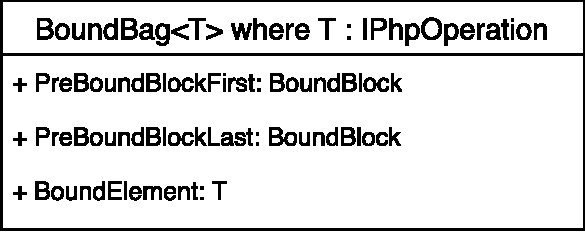
\includegraphics[scale=0.75]{../img/5_3_BoundBag}	
	\caption{Bound bag.}
	\label{fig5.3:BoundBag}
\end{figure}

With the container, we need to change the public public API of the \emph{SemanticBinder} so that it exposes methods that return this \emph{bound bag} instead of a plain bound expression or bound statement. We cannot replace the original methods, however. They are not used just externally but also internally by the \emph{SemanticBinder}. It uses them to bind individual nodes one by one when it is asked to bind a whole expression tree. And in these situations we want them to return plain old bound elements. More about that later.

Instead, we can make the original methods private and add new public methods, let us call them \emph{BindWholeStatement} and \emph{BindWholeExpression}, that will return a \emph{bound bag}. For now, they can call the private ones and only wrap their results into \emph{bound bags} with empty \emph{pre-bound graphs} (\autoref{fig5.3:BindWholeExpr}). We will get back to them later too. Before that, however, we need to fix all the external calls to the - now private - methods and change them to accept a bound bag instead of a sole bound item

\begin{figure}[H]
	\centering	
	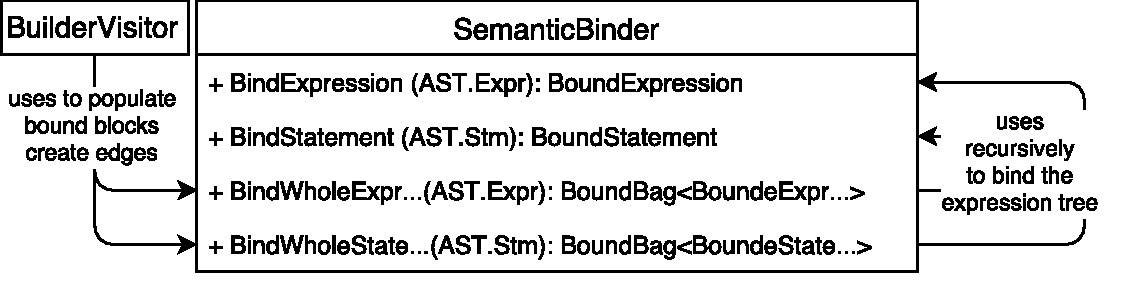
\includegraphics[scale=0.75]{../img/5_3_BoundWholeExpression}	
	\caption{Builder visitor's and semantic binder's relationship.}
	\label{fig5.3:BindWholeExpr}
\end{figure}

The fix is straightforward for statements. The original \emph{BindStatement} method is externally called just once, when the \emph{BuilderVisitor} needs to bind a new statement to add it to its \emph{current bound block}. To support getting a \emph{bound bag} instead of plain bound statement we need to connect its \emph{pre-bound graph} before adding the bound statement to the \emph{current block}. That means creating a simple edge between the \emph{current block} and the \emph{first pre-bound block}, and setting the \emph{last pre-bound block} as the new \emph{current block} (\autoref{fig5.3:BindNewStm}). As the one, into which the bound element will get added.

\begin{figure}[H]
	\centering	
	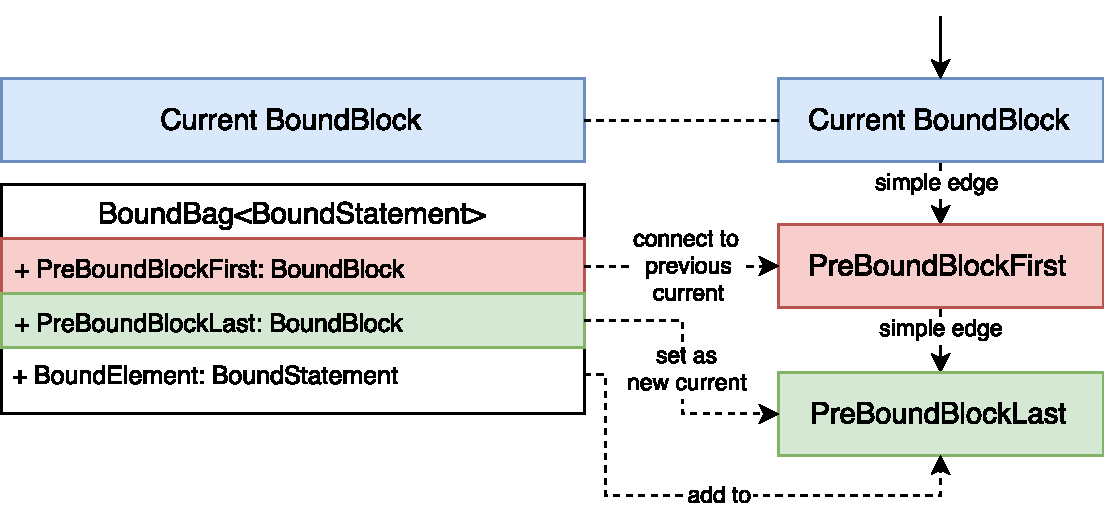
\includegraphics[scale=0.75]{../img/5_3_newStatement}	
	\caption{Connecting a bound bag as a new statement.}
	\label{fig5.3:BindNewStm}
\end{figure}

The situation regarding expressions is a bit more complicated. \emph{BindExpression} is externally called in three situations. When another symbol needs to bind a constant, for example a parameter its initializer. When a \emph{BuilderVisitor} needs an expression representing a reference to a synthesized but user accessible variable, such as \emph{foreach}’s key and value variables. And lastly, when also a \emph{BuilderVisitor} needs to bind an expression for some edge, like a \emph{condition expression} for \emph{condition edge}.

The first two cases are relatively easy to adapt to the bound bag. Both variable references and constants are guaranteed to not to include a \emph{yield} and thus to not to produce a \emph{pre-bound graph}. Therefore, we can retrieve the bound expression from their bound bags and leave the implementation without any further modifications.

The third one is a bit more complicated. There are four instances in which the \emph{BuilderVisitor} asks the \emph{SemanticBinder} to bind a full unrestricted expression. For a \emph{switch edge}’s switch and case values, \emph{condition edge}’s condition, and \emph{foreach}’s enumeree. All of them are problematic because when new edges are being created, it is hard to say what the \emph{current bond block}, to which the \emph{pre-bound graph} should be connected, actually is.

Generally, there are two possible answers for that. One is enriching each of these edges with special branches for these expressions’ pre-bound blocks. On one hand, this is more systematic, it clearly maps the intend to the semantic structure. On the other, it increases complexity for all of these edges’ instances to support a feature used only by generator methods. The second way is to choose any appropriate block and connect the \emph{pre-bound graph} to it. An appropriate block means any block that the \emph{pre-bound graph} can be connected to with the condition that emit of the result must produce a program with correct PHP semantics.

For \emph{condition edge}’s condition, \emph{foreach}’s enumeree, and \emph{switch}’s switch value expressions one such block is their edge’s \emph{source block}. That it the block, the edges connect to as their starting point and also usually the last \emph{current block}. It is a good choice, because these expressions are the first things executed within their respective edges and so the block directly before said edges is also a block directly before them.

Thus, for these three the solution is to take the \emph{first pre-bound block}, connect it to the edge’s \emph{source block}, set the \emph{last pre-bound block} as the new \emph{source block} (\autoref{fig5.3:BindIfEdge}), and continue the edge creation using a bound expression as before.

\begin{figure}[H]
	\centering	
	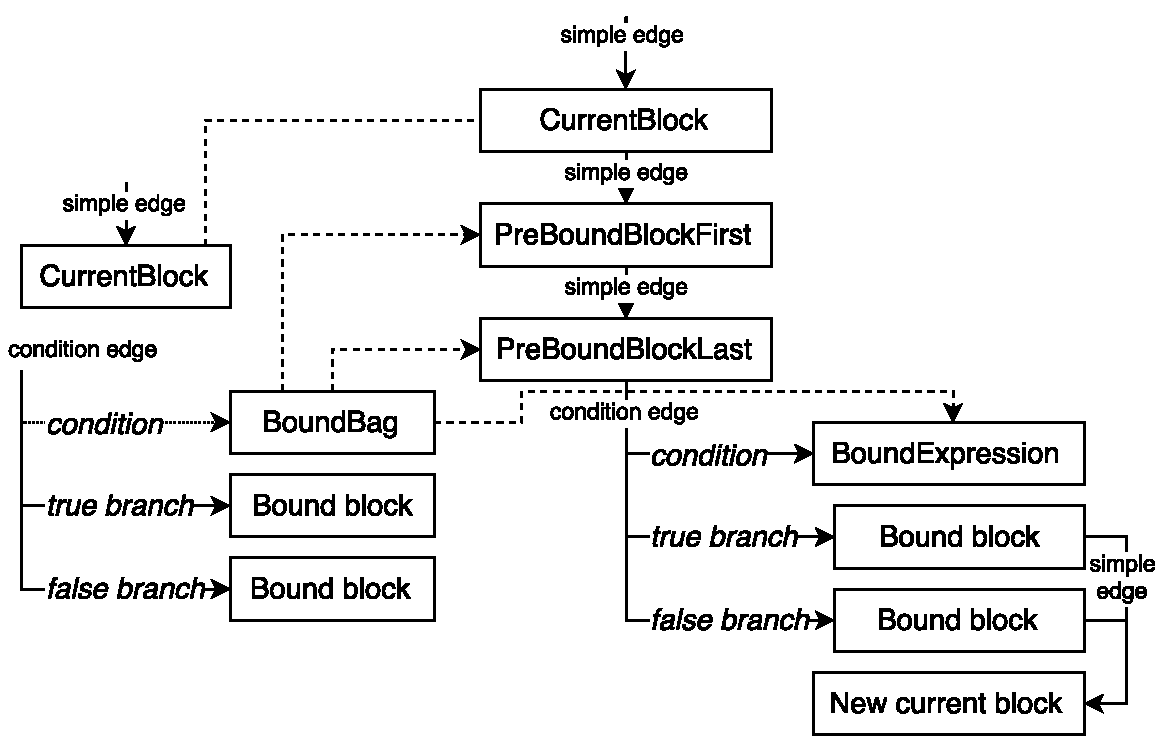
\includegraphics[scale=0.70]{../img/5_3_newInIfEdge}	
	\caption{Connecting a bound bag as a condition edge's condition.}
	\label{fig5.3:BindIfEdge}
\end{figure}

This approach is, unfortunately, not applicable for the fourth case, a \emph{switch edge}’s (\autoref{fig5.3:SwitchEdge}) case value expression. This is an expression representing the value a \emph{switch value} is compared to for each case block. The reason is, that the \emph{case value expression} is executed neither in the beginning of the edge or directly after some other block, so there is simply no block to connect the \emph{case value}’s \emph{pre-bound graph} to. With it we need to go the first way and implement a support for \emph{pre-bound blocks} directly on the edge. Actually, not on the edge itself but on the \emph{case block} the \emph{switch edge} points to.

That itself is not that complicated. We can remember the whole case value bound bag in the case block and emit the \emph{pre-bound graph} directly before the case value condition. The issue is, that the evaluation stack is not guaranteed and actually never is empty at that point. Because only one case block can be taken in PHP switch, Peachpie actually keeps the \emph{switch value} on the evaluation stack from the beginning of a switch edge evaluation and goes one \emph{case block} after another comparing their \emph{case values} with it.

Therefore, if a particular case block has any \emph{pre-bound graph} we need to pop the \emph{switch value} first and then, after emitting its \emph{pre-bound graph}, load it again. To not to evaluate the \emph{switch value} multiple times, we also must replace it with a temporal variable. A temporal variable into which the \emph{switch value} is saved, or captured in other words, in the very beginning.

\begin{figure}[H]
	\centering	
	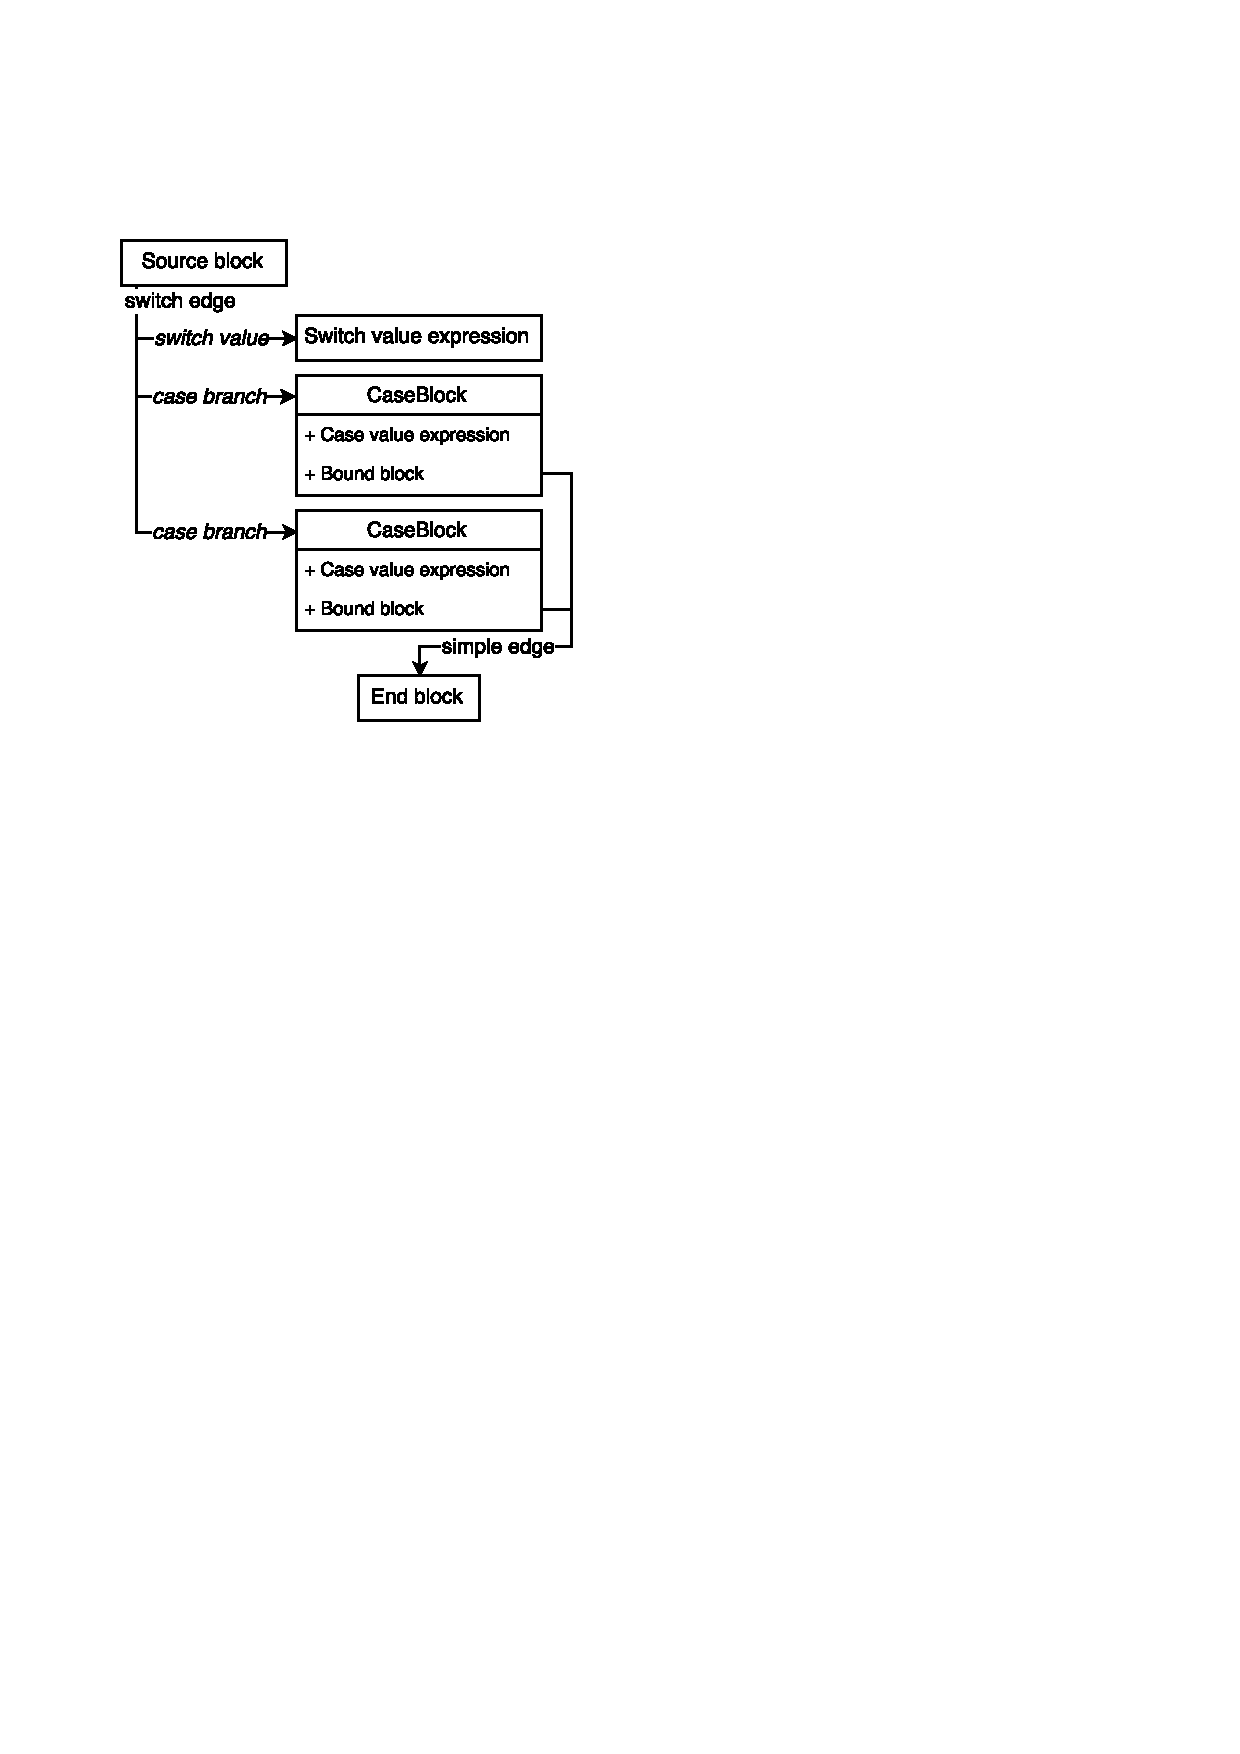
\includegraphics[scale=0.75]{../img/5_3_switchEdge}	
	\caption{Switch edge diagram.}
	\label{fig5.3:SwitchEdge}
\end{figure}

There are certain optimizations that can be done as part of this process. For example, we do not need to do the whole switch value saving if it is a constant. They are, however, implementation details. 

\subsection{Capturing branches with yields}

Now that all external components can handle bound bags with pre-bound blocks, it is time to actually implement the algorithm that creates them. The implementation is based on one core principle. 

When the semantic binder is asked to bind an AST, be it an expression or a statement, it first of all prepares an empty \emph{first pre-bound block} for the item that will be bound. Then, it proceeds with binding the element, its children, and so on recursively as already described in the semantic graph chapter. And when any of these nodes is under any path between a \emph{yield} and the root of the currently bound expression tree, it creates its semantic representation but does not simply return it. Instead, the semantic binder constructs a new \emph{assignment statement} that sets the bound expression to a new temporal variable, puts said statement into the current \emph{pre-bound block}, and returns a \emph{read expression} from the temporal variable (\autoref{fig5.3:CaptureWithYield}). That way the read from the temporal variable ends up in the resulting expression tree instead of the bound expression and the bound expression becomes captured. And when the AST finishes binding it gets returned as part of the bound bag’s pre-bound graph.

\begin{figure}[H]
	\centering	
	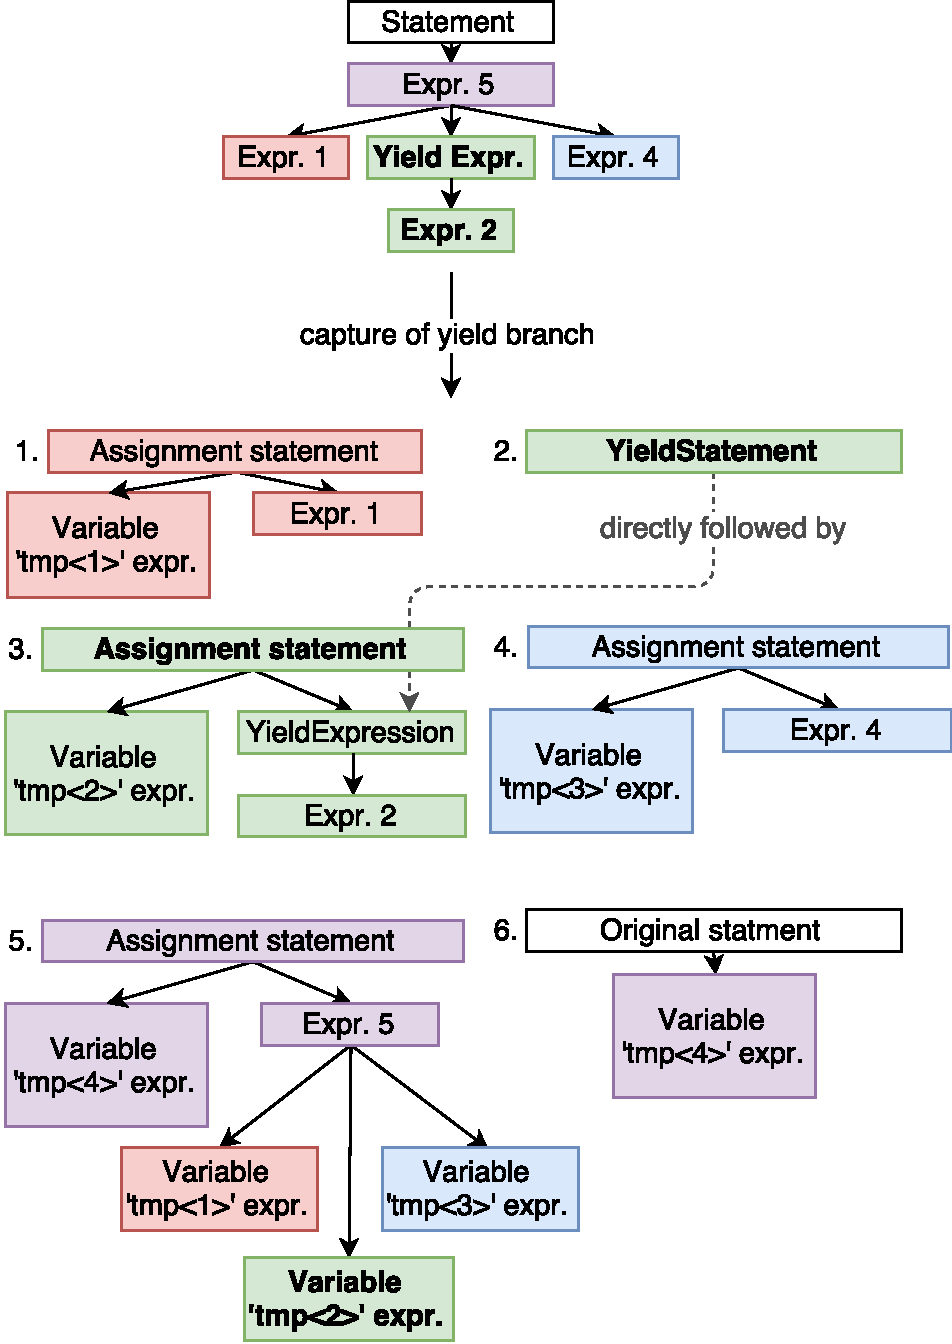
\includegraphics[scale=0.75]{../img/5_3_branchesWithYields}	
	\caption{Capturing a branch with a yield.}
	\label{fig5.3:CaptureWithYield}
\end{figure}

Two things are needed to support such behavior, the ability to determine whether any particular node is under a path between the current expression tree’s root a \emph{yield} and a way to keep \emph{pre-bound blocks} while an expression tree for an AST is being binded. Before going into details on implementing each of these, however, let us first take a look at a small modification we have made to the algorithm in comparison to the one described in a previous chapter\footnote{Chapter \ref{AlghTheory}}.

\subsection{Correctness of modified capturing algorithm}

The actually implemented algorithm captures all branches that start with children of elements on the \emph{root-yield} path instead of only the children to the left. It also captures branches starting on the path itself, after all they are children of some elements one level higher in the path. The reason for that is, that neither the AST nor the semantic tree has a generic notion of left to right ordered children. Therefore it would be hard to determine whether a current element is to the left of the path or to the right. This change, however, does not alter the fact that the transformation keeps the original order of execution.

The implemented version captures a superset of branches the theoretical algorithm did. The ones on top of that are, as the original were, still captured and prepended in a post-order, which guarantees the correct order of execution. In essence, the ones to the right will get prepended and thus executed only after those to the left, and the ones on the path itself only after all their children.

The capturing is done in a post-order order because following statement holds true. The \emph{SemanticBinder} itself operates as a depth first search and the capturing is the last part of a node’s binding process. When an element is being bound, its semantic representation is created first, part of which is fully binding its children from left to right, and only after that, the node itself might get captured and subsequently returned as bound. The thing is, that as part of the children's’ binding process, they themselves might get captured and therefore prepended first. 

Capturing both a child node and its parent’s, which is something that happens with our version for almost all elements on the path, is not a problem either. It creates two prepended statements, first the child’s and then the the parent’s as proven above. The parent’s prepended statement will contain an expression tree with the children’s original branch replaced by the children’s temporal variable (\autoref{fig5.3:CaptureWithYield}). And the original expression tree will contain the parent’s branch replaced with the parent’s temporal variable. Since the children’s prepended statement is first, it will get executed before the parent’s. Thus the execution order will remain correct.

\subsection{Creating and keeping the pre-bound graph}

Now that we are sure our modified version is still correct, let us go back and implement the two things we need for the algorithm to work. First, we will take a look at creating and keeping the pre-bound blocks while binding an AST.

The keeping part is straightforward, we only need two new fields with references to bound blocks on the \emph{SemanticBinder}. Two because, as we have discussed before, we need both the first and the last block for the eventually returned \emph{bound bag}. The reference to the last bound block can also serve as the \emph{current pre-prebound block} into which new captured branches are added.

The actually complicated part is getting new empty bound blocks. While the \emph{SemanticBinder} could just create brand new bound blocks instances itself, there is a small problem with the fact that bound blocks are in fact ordered. They all have an ordinal number that represents where - in comparison to other bound blocks - do they fit within the original source file. The higher their number the further the code they represent was in the original source code. For example imagine an if statement (\autoref{fig5.3:BlocksOrdinal}): the block before the if itself must have the smallest ordinal number, the true block higher, the else block higher still, and the block directly after the highest.

\begin{figure}[H]
	\centering	
	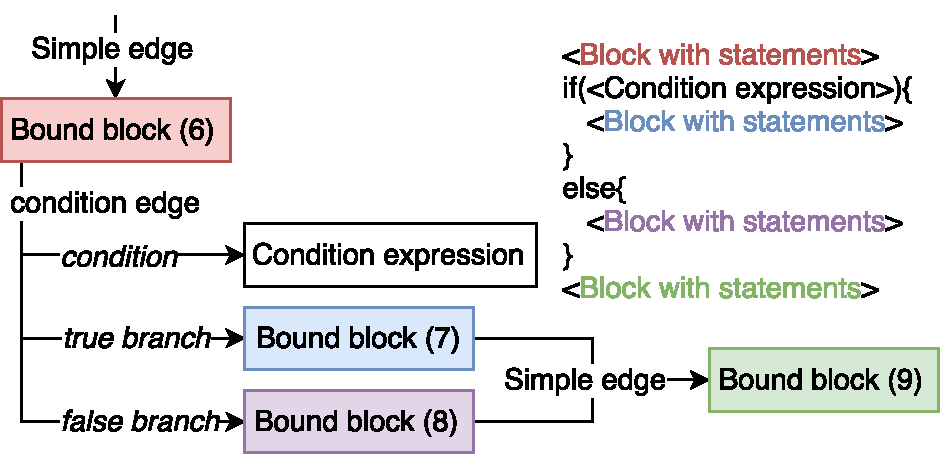
\includegraphics[scale=0.75]{../img/5_3_blockOrdinal}	
	\caption{Ordinal number of bound blocks.}
	\label{fig5.3:BlocksOrdinal}
\end{figure}

The problem is that the \emph{SemanticBinder} does not know the last ordinal number the \emph{BuilderVisitor} used to create its \emph{current bound block}. And so, it does not know what ordinal number to use for a new \emph{pre-bound block} that will represent the current statement’s or expression’s \emph{pre-bound graph}.

It is true that the \emph{SemanticBinder} could create all these \emph{pre-bound blocks} with an ordinal number 0 and then the \emph{BuilderVisitor} could fix them as part of the phase that connects the \emph{pre-bound graph}. That would, however, require creating a new component that could traverse the graph and would know its topology. While the \emph{BuilderVisitor} knows how to create the semantic graph, it does not have generic tools to traverse it or to update its nodes’ ordinal numbers.

It was also briefly considered to simply pass the last used ordinal number with each to call the \emph{SemanticBinder} and then return the new one as part of the \emph{bound bag}. This approach was not chosen in the end, however, because it breaks the abstraction separation between two relatively independent components.

Thus, it was chosen to offload the creation of new bound blocks to the \emph{BuilderVisitor} instead. As part of an initialization phase, the \emph{SemanticBinder} takes a reference to the \emph{BuilderVIsitor} and, when needed, uses it to get new bound blocks with the correct ordinal number. The only requirement for this to work is to ensure following invariant stays true. When an element is being bound, the last block created by the builder visitor must be the block directly before the element. And as it turns out, this is an already existing invariant in the Peachpie compiler.

With this approach, the \emph{SemanticBinder} can get a new empty bound block with the correct ordinal number without having to actually know or care about ordinal numbers. For now, this is relevant only for the one initial bound block that gets created in the beginning of a binding process, is used as the storage for all the captured branches, and in the end gets returned as part of the \emph{bound bag}. Later, it will become more important when conditioned branches come into play because they will require getting a number of bound blocks for the \emph{pre-bound graph}.

\subsection{Path between the root and yields}

To be able to tell whether an element is under a path between the root of the current expression tree and any \emph{yield}, we need to have the paths first. While it would be possible to simply traverse the full graph with a depth first search and record the path whenever we find a \emph{yield}, there is actually a simpler way. 

As part of the AST the parser returns a list of references to all found \emph{yield expressions}. Due to that, we only need to go through this list, assign individual \emph{yield}s to their respective method symbols, and realize these paths. The first part of the process are trivial busywork and thus will not be discussed in detail. 

Since the paths are needed before any node from a method is bound, the realization is best done as part of the method’s \emph{SemanticBinder}’s initialization. The realization itself is a two steps process. First, the abstract syntax nodes representing the \emph{yield}s must get into the \emph{SemanticBinder}. They can simply be passed there from the routine that creates the method’s CFG and thus also initiates its \emph{SemanticBinder}. 

The second step is actually creating the paths. For that, it is useful to know that all syntax nodes have a generic reference to their parent node. Thus, it is quite easy to traverse the syntax graph upwards, which is all we need to do. We can start with every \emph{yield expression} and just go upwards in the graph until we get to a node representing the enclosing method, recording the path along the way. Do note that paths created this way are not the paths between a \emph{yield} and its expression tree’s root but a \emph{yield} and the method’s root. While it might look as a minor thing it will be important.

Now that we have the paths for all \emph{yield}s within a method, let us take look at the mechanism to find out whether a node is under any of said paths. Just checking whether the parent of a currently bound abstract syntax node is within any recorded path is not enough. It is not enough precisely because the paths do not stop at expression tree roots but instead continue to the methods’ roots and as such include things like edges. 

For example (\autoref{fig5.3:Path}), if a \emph{yield} was in a true branch of an \emph{if edge}, the path would also contain the \emph{if edge}’s syntax node. Therefore, the first node of the \emph{if edge}’s \emph{condition expression} would report as being under the path despite the fact it actually is not under the path we care about, the path between a yield and its expression tree’s root.

Therefore, we need a more nuanced mechanism. A good observation to make is, that we know about each expression tree’s root. It is the node passed to the public \emph{SemanticBinder}’s methods that invoke the binding process of an AST, the \emph{BindWholeExpression} and \emph{BindWholeStatement}\footnote{Chapter \ref{BindMultiple}}. With this knowledge, and the fact that the binding process is essentially a depth first search, we can solve this issue through a new \emph{level} field on the \emph{SemanticBinder}. A \emph{level} field that represents how deep we are under the closest \emph{yield-root} path in the currently bound expression tree (\autoref{fig5.3:Path}).

\begin{figure}[H]
	\centering	
	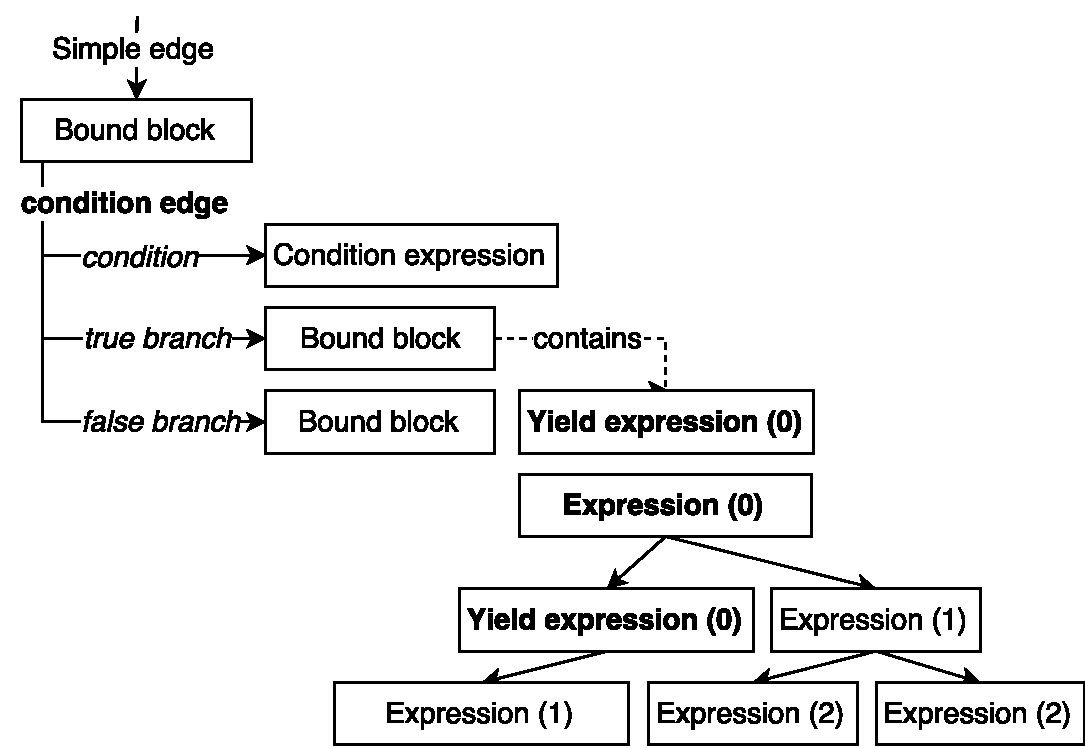
\includegraphics[scale=0.75]{../img/5_3_path}	
	\caption{Path between a yield and expression tree's root.}
	\label{fig5.3:Path}
\end{figure}

When the \emph{SemanticBinder} starts binding an AST through any of its public methods, the \emph{level} is set to -1, representing that there is no known relevant path above. There cannot be one because at that point the current node, that is being bound, is the expression tree’s root. 

Then, in the beginning of each of the methods that bind the tree’s individual nodes, \emph{BindStatement} and \emph{BindExpression}, the \emph{level} is saved to a local variable and the field is updated. The update consist of two operations. First, if the current \emph{level} is not $-1$, it is increased by one, indicating that we are one level deeper. Second, it is checked whether the current node’s parent is part of any path and when it is, the \emph{level} is set to $0$. 

After setting the \emph{level}, a semantic representation of the node is created, and its children are bound, potentially also captured. Then, the current \emph{level} is checked. If it is $1$ or $0$, which means the node is either on the path or directly below it, the just bound node gets captured as described before\footnote{Chapter \ref{Capture}}, adding a statement that assigns it to a new temporal variable into the \emph{current pre-bound block}. Finally, the original \emph{level} is restored from a local variable and either the bound node or, if it was captured a read from its respective temporal variable, gets returned.

\subsection{Conditioned branches}

With that, we have all the building blocks needed to have an implementation that handles yields as expressions in every situation except for when the yield is in a conditioned branch. That means either a branch of a \emph{conditioned expression} or a short-circuit evaluated \emph{binary expression}.

For a \emph{conditional expression} there are two \emph{conditioned branches} and one separate \emph{condition branch} that dictates which of the first two branches will get evaluated. For short circuit evaluated \emph{binary expressions} there only two children branches in total. A \emph{condition} one and a \emph{conditioned} one. The rule is that it the \emph{conditioned} is evaluated only if the first one, the \emph{condition} one, has not already satisfied the rule of the short circuit evaluation.  

We have already discussed the theoretical approach to solving this problem\footnote{Chapter \ref{shortCircTheory}}. Its implementation is following. When binding an element with a conditioned branch, the branch is bound as a standalone expression tree. The result of the branch’s binding, its \emph{bound bag}, then used to determine whether the branch contains a \emph{yield} or not. The key is whether its \emph{pre-bound graph} is non-empty. When it does contain a \emph{yield}, said \emph{pre-bound graph} is connected to the \emph{last pre-bound block} of the currently bound expression tree through a \emph{condition branch}. A \emph{condition branch} that uses the same \emph{condition expression} that guards the branch (\autoref{fig5.3:YieldInCond}). This effectively ensures the the \emph{pre-bound blocks}, constituting the \emph{pre-bound graph}, of the branch are evaluated only when the branch is, in essence when its condition is true.
 
The issue with multiple evaluations of the \emph{condition expression}, that can happen because now we have the condition both in the original expression and in the \emph{condition edge}, is solvable through a simple observation. When the \emph{conditioned branch} includes a \emph{yield}, the expression that the branch stems from must be on the path between it and the expression tree’s root. Therefore, the \emph{condition expression}, that starts from the same node the \emph{conditioned branch} does, is guaranteed to be directly under said path. 

With that knowledge we can capture the \emph{condition expression} while binding the shared parent node and reuse its temporal variable in the both the expression’s condition, i.e. the original position, and the branch’s \emph{pre-bound graph}’s \emph{condition edge}. Since the \emph{condition expression} is guaranteed to be under the path, all expressions to the left from it has already been captured and prepended and so the order of execution stays correct.

\begin{figure}[H]
	\centering	
	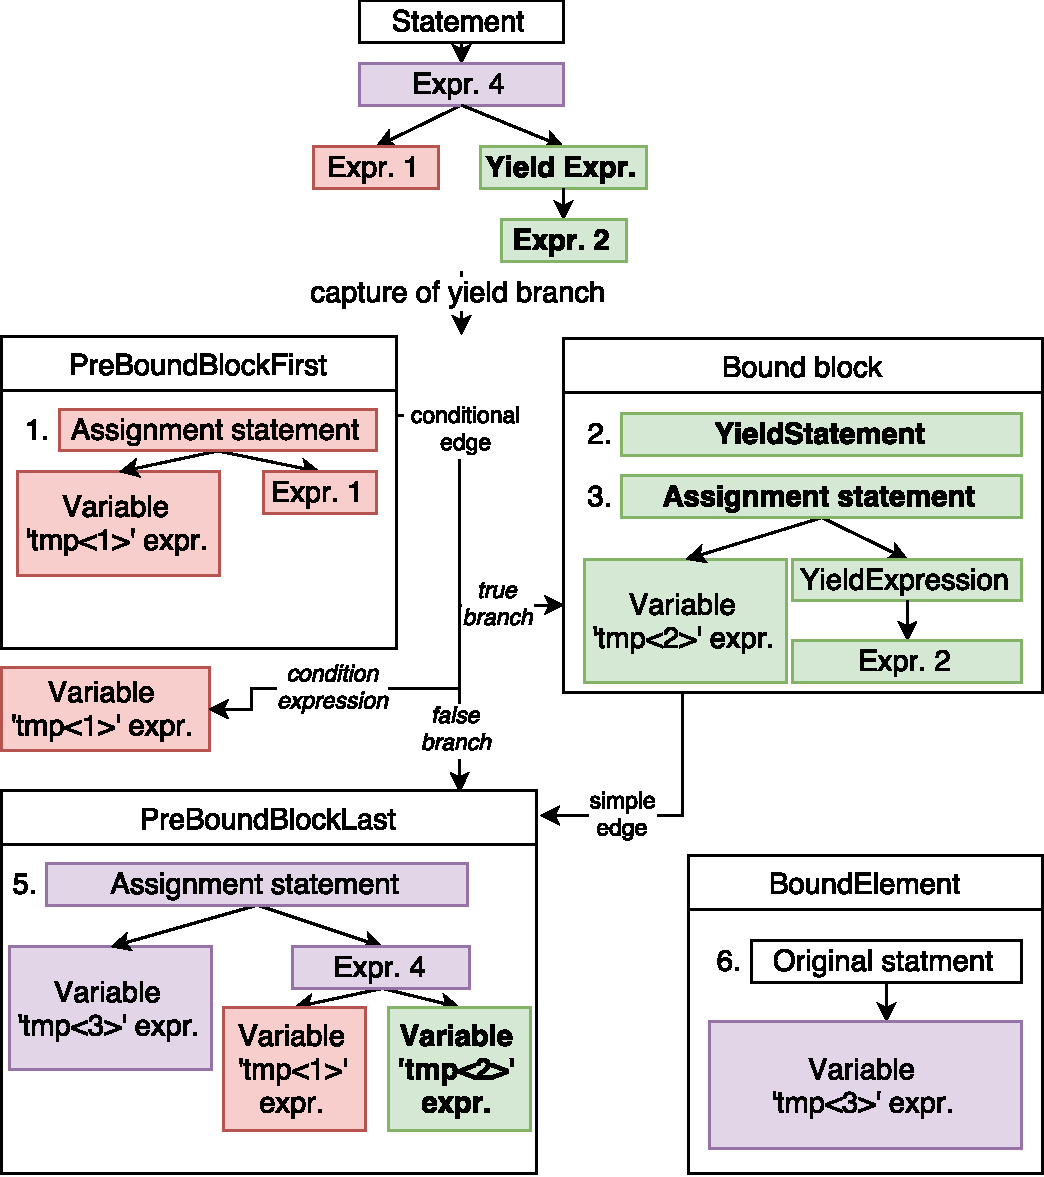
\includegraphics[scale=0.75]{../img/5_3_yieldInCond}	
	\caption{Capturing a yield in a conditioned branch.}
	\label{fig5.3:YieldInCond}
\end{figure}

Now the only thing that remains to be described is the way to bind the branch as a standalone expression tree in the middle of binding its enclosing one. One possible way is to save both references to the \emph{pre-bound blocks} on the \emph{SemanticBinder} to local variables, initialize them to a default value, and proceed with binding the branch through normal means. When it is done, capture the branch’s \emph{pre-bound graph} from the now re-populated \emph{pre-bound block}s references, construct its bound bag, restore the \emph{pre-bound block}s references to their original values, and return the bag. That way the solution works even with nested conditioned branches.

\subsection{Implementation remarks}

In previous sections we have presented a high level discussion about the implementation of an algorithm that lowers generator methods using only relatively small modifications to a \emph{SemanticBinder} and a \emph{BuilderVisitor}. While they are more of implementation details, there are a few remarks that could be useful for the reader but do not fit into any previous chapter due to either being too specific or requiring knowledge about the system as a whole.

Not all expressions need to be captured when the algorithm signals they should. Since the capture of non-yield branches only ensures the correct order of execution, it is redundant for expressions that have no side effects and whose value cannot change in time. While these properties are hard to prove for an arbitrary expression they are guaranteed to be true for two specific types of expressions: a \emph{constant expression}, such as a number literal, and an expression that has a constant value resolved by the compiler. Thus, branches consisting of only these types of expressions can be omitted from capturing. 

To mitigate any possible performance penalties for non-generator methods and separate generators specific code, it is possible to have two semantic binders. One that serves as the basis and is used for all normal methods and the other that inherits from it and handles generator methods.

The only change we need to make to the basic one, in comparison to the original pre-generators \emph{SemanticBinder}, is to create the new public methods for binding expressions and statements and make them return \emph{bound bag}s with empty \emph{pre-bound graphs}. In the generators specific \emph{SemanticBinder} we can override both these methods and the ones that bind the AST’s individual nodes and put all the generators specific logic there. 

The question which \emph{SemanticBinder} to use for any particular method has a straightforward answer. Since a \emph{SemanticBinder} for a method is initiated only after the method’s AST has been created by the parser, it is already known whether the method contains any yields and as such if it is a generator method. With that knowledge we can simply create the appropriate \emph{SemanticBinder} and pass it to the method’s respective \emph{BuilderVisitor} to use. 

There is obviously more to the implementation than described in the chapters above. To name a few, we have completely left out the changes required to make return type analysis work, complexities related to throwing into and rewinding generators, all logic associated with generator’s return value, or how Peachpie keeps the list of method’s yields to be able to construct the jump table in the beginning of a generator’s \emph{next} method. All of these are, however, details that might, and most probably will, change in near future as the Peachpie project matures. Thus they do not provide any value for a reader that might want to either understand why peachpie works a certain way or implement a similar feature. And for those that are interested in line by line explanation the source code, or at least the part implemented as part of this thesis, is commented in detail. 


\section{Yield in exception handling blocks}

Now that we have fully described the implementation of generators within the boundaries set in the introduction, let us briefly look at possible ways to expand them. Specifically, at dealing with with \emph{yield}s in exception handling blocks. Due to the extent of this thesis and the complexity of arbitrarily placed \emph{yield}s\footnote{\citep{CSharpYieldCatch, CSharpYieldFinally, CSharpYieldTry}} we will neither propose a full solution nor describe an actual implementation. Rather, the following chapter will outline a possible approach that might serve as a starting point for possible future work.

The implementation described in previous chapters cannot handle yields in exception handling blocks itself because CIL does allow neither jumping into an exception handling block nor returning from it\footnote{Chapter \ref{CILExc}}. And the core principle of our approach is transforming yields into jump target labels and return statements.

We also cannot take a direct inspiration from Roslyn. While C\# does not forbid \emph{yield}s in exception handling blocks completely, it allows them only in a very limited way that is not really useful to us. It would theoretically be possible to take a look at how Roslyn handles \emph{await}s in said blocks, because methods with \emph{await}s are also lowered to state machines \citep{CSAwait}, but that approach was deemed unnecessarily complex for our needs. However, anyone considering actually implementing our proposed solution should use it as a resource.

\subsection{Yields and exception handling blocks in PHP}

Before going into details, we need to define what \emph{yield}s in individual exception handling blocks even mean. A \emph{yield} in any of these blocks, be it \emph{try}, \emph{catch}, or \emph{finally}, has the same basics semantics. It returns from the function and serves as a possible continuation point for whenever the generator’s \emph{next} method is invoked again. Despite that, there are certain situations in which the \emph{yield} behaves abnormally.

When there is a \emph{try} block but no appropriate \emph{catch} block and an exception is thrown, the exception is saved and does not actually truly appear until after a potential \emph{finally} block associated with the \emph{try} block finishes. And since the possible finally block can contain \emph{yield}s itself, it is possible for an exception to actually appear and crawl out of the generator’s \emph{next} method only after several advancements of the generator. 

There is also a special behaviour associated with \emph{finally} blocks. When an execution of a generator stops in a block that has an unfinished \emph{finally} block associated, be in in a \emph{try}, \emph{catch}, of the \emph{finally} block itself, and the generator is about to be deleted by the GC, the \emph{finally} block still gets run. At that point, however, it cannot contain any further \emph{yield}s. If it does, a runtime error gets thrown.

\subsection{Solution in Peachpie}

The core idea of our proposed approach is, that we can effectively emulate the exception handling process without having to worry about the aforementioned limitations of the native one. This has some obvious drawbacks. Most importantly, it introduces a non-trivial performance hit for both a situation when an exception is thrown but also for when it is not. Depending on implementation details, the hit can either be a bit smaller or bigger but it will always be there when trying to emulate the process without using native primitives provided by the CLR.

The emulation is based on three principles. The generator instance holds the information in which exception handling block the execution currently is. Both starts and ends of all exception handling blocks get transformed into specific series of statements that do two main things: keep the aforementioned information updated and they serve as labels for potential jumps. Last but not least, the whole transformed \emph{next} method is wrapped in one giant \emph{try} block with a \emph{catch} in the end. A \emph{catch} block that retrieves the information regarding which exception handling block the execution was last in and acts accordingly. 

Since there is only one giant \emph{try} block, the whole already described implementation of the \emph{next} method can be in it. Therefore, it can contain both the initial jump table and the whole generator’s code including all \emph{yield}s. That means, there do not have to be any jumps into or from exception handling blocks, only within the big one. And regarding \emph{return}s, they can simply be replaced with the special instruction to leave a \emph{try} block and then a \emph{return}.

All starts and ends of exception handling blocks must do one thing, update the information about the current exception handling block. In addition to that, the starts of \emph{catch} blocks must include a jump label, possible conditional jump to the next catch handler for filtering only the appropriate exception type, and an unsetting of a saved exception. More about the saved exception later. The starts of \emph{finally} blocks must contain a jump label as well, and the ends should close with a throw of a saved exception, if there is any.

The one global catch block should do following. It should retrieve the exception handling block that was just being executed. If it was a \emph{try} block or a \emph{catch} block with associated \emph{finally} block, it should save the exception on the generator instance, otherwise it should just rethrow. Then, it should figure out where to jump next, in essence where to continue with the execution. If the last executed block was a \emph{try} block, it should jump either to its \emph{catch} block label or its \emph{finally} block label. If it was a \emph{catch} block, then to the \emph{finally} block label. Lastly, just before jumping it should update and correct the information about the current exception handling block, the execution is just leaving one, after all.

To support the situation in which a generator object is going to be collected and its \emph{finally} blocks should run, the generator type can implement an explicit \emph{IDisposable} interface. Then in the dispose method, it can gather the exception handling blocks its execution stopped in and run all of their finally blocks. An explicit \emph{IDisposable} interface is required instead of just using CLI finalizers because of different GC semantics between the CLR and PHP \citep{GenPHPRFC, CSharpEcma}. 

It is guaranteed that the finally blocks are triggered immediately after the last reference to the generator instance disappears in PHP. The same thing cannot be said for CLI. There is simply no way to get notified immediately after the last reference to an object disappears. Also, having arbitrary code in finalizers is highly discouraged. Since they can run in an arbitrary order it is possible that objects the generator instance might be pointing to, and that might be used by the code in the finally blocks, could have already been collected and their references set to null by the time generator’s finalizer runs. 

The idea outlined above is in no way comprehensive and misses a number of important details that would need to be ironed out before implementing it. In spite of that, it should serve as a good starting point.

\section{Future work}

Even though this thesis comes with a full featured implementation, there is obviously a room for further expansion. And since the project is, as of writing this thesis, still in a rapid development, it is not only possible but very probable that many of these possible follow ups will get implemented soon. That, however, does not mean they should not be noted here.

In addition to implementing the aforementioned yields in exception handling blocks, the other largest opportunity for improvement lies in employing lowering more throughout the compiler. Both the yield statement and the yield expression could be largely replaced by a lowering into lower level language constructs (\autoref{fig5.5:YieldInCond}). While having standalone nodes was very useful for prototyping and debugging reasons, using already existing means, the rest of the infrastructure understand, is better in the long run. 

\begin{figure}[h]
	\centering	
	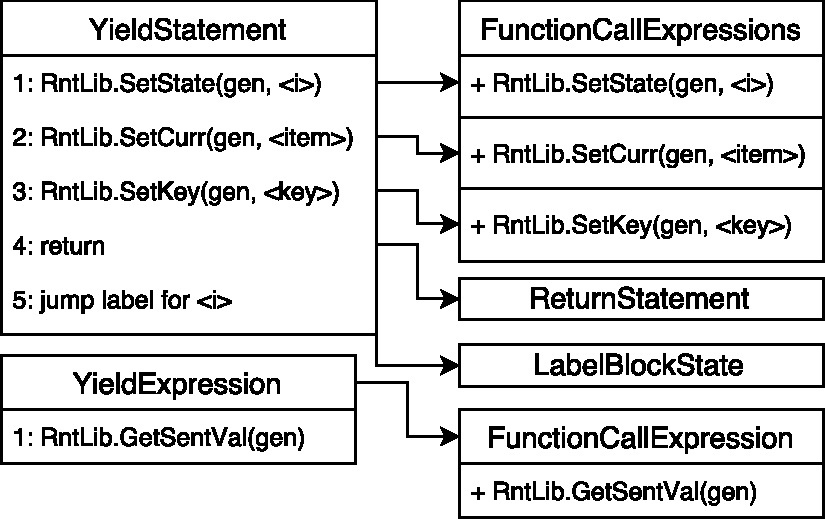
\includegraphics[scale=0.75]{../img/6_6_yieldLowering}	
	\caption{Possible lowering solution to a yield expression and a yield statement.}
	\label{fig5.5:YieldInCond}
\end{figure}

Lowering could also be used instead of having a custom path in the emit method of a routine symbol for generators\footnote{Chapter \ref{MethdSymbol}}. For generator methods, the semantic binder could simply do two things. First, construct a semantic graph that would represent a generator’s instantiation, initialization, and return and then use the graph as the body of the actual generator method. Second, synthesize a separate routine symbol for the generator's next method and bind the original generator method’s body for it.

While not particularly interesting or complex, a \emph{yield from} statement could also be implemented. It provides a way to specify that at some point a generator should yield elements from some iterator until it exhausts it and only then move on to the next \emph{yield}.

There is also great potential in expanding the available code diagnostics. Peachpie compiler could, for example, warn about using \emph{yield}s in finally block, short-circuit evaluated branches, or other potentially problematic places.




\chapter*{Conclusion}
\addcontentsline{toc}{chapter}{Conclusion}

In previous four sections we have first described the fundamental concepts required for understanding this thesis, then designed an algorithm to support our feature, provided an overview of said algorithm's implementation, and, in the end, proposed possible expansions.

While the work on generators support within the Peachpie compiler is by no means done, the shipped implementation provides a good foundation that can stand on its own. It brings support for all generator’s features, except for yields in exception handling blocks. And while that is an useful feature, it is a more of an extension of generators than its fundamental building block. Other than that our implementation mimics the reference semantics faithfully, while expanding upon the featureset usual in other CLI based languages such as in C\#.

The goal of using as much existing architecture as possible and not creating unnecessary abstractions just for generators was also achieved. While there is still room for an improvement, all generators specific code is either cleanly separated or abstracted to be used by other compiler components as well. 
Lastly, while not an explicitly stated goal, the compilation of generators is efficient. It does not introduce any new semantic tree or syntax tree traversals and only slightly increases the memory required for the binding phase. Due to the separation of all specific logic to a special binder, it has absolutely no impact on binding, and thus compiling, non-generator methods.

In conclusion, this thesis and the attached implementation fulfill all goals set by both the thesis assignment and us in the introduction section. On top of that, it brings a self-contained functionality to a popular open source project.

%%% Attachments to the bachelor thesis, if any. Each attachment must be
%%% referred to at least once from the text of the thesis. Attachments
%%% are numbered.
%%%
%%% The printed version should preferably contain attachments, which can be
%%% read (additional tables and charts, supplementary text, examples of
%%% program output, etc.). The electronic version is more suited for attachments
%%% which will likely be used in an electronic form rather than read (program
%%% source code, data files, interactive charts, etc.). Electronic attachments
%%% should be uploaded to SIS and optionally also included in the thesis on a~CD/DVD.
%%% Allowed file formats are specified in provision of the rector no. 23/2016.
\chapwithtoc{Attachments}

Attached to this thesis is a snapshot of Peachpie project’s git repository. It contains not only the implementation that was done as the practical part of this thesis but also the rest of the complete project. A more up to date version can be found on github\footnotemark.

To query only commits done by the author of this thesis please filter out author \emph{Petr Houška} or email \emph{houskape@gmail.com}.

\footnotetext{
	\href{https://github.com/peachpiecompiler/peachpie}{github.com/peachpiecompiler/peachpie}
}

\secwithtoc{Compilation}
The project’s only implicit dependency is .NET Core runtime and optionally its CLI SDK. If you want to compile the project yourself you can download both of them from the official site\footnotemark, for Linux, Windows, or MacOSX.

After obtaining the .NET Core SDK please navigate to the folder with the Peachpie repository in your favourite terminal and:

\begin{minted}[breaklines=true]{text}
dotnet restore  //download all external packages required
dotnet build    //build the complete solution
\end{minted}

\footnotetext{
	\href{https://www.microsoft.com/net/download/core}{microsoft.com/net/download/core}
}

\secwithtoc{Structure}
There are three components relevant for this thesis within the repository. The compiler binaries, the compiler implementation, and the generators tests. Below are listed paths to them and in case of the compiler’s implementation also to some files containing the majority of our work to support generators.

\begin{enumerate}
	\item \label{peach}src/Compiler/peach	
	\item src/CodeAnalysis
	\begin{enumerate}
		\item ./Semantics/SemanticsBinder.cs
		\item ./Semantics/Graph/BuilderVisitor.cs
		\item src/Peachpie.Runtime/std/Generator.cs
	\end{enumerate}
	\item tests/generators
\end{enumerate}

\secwithtoc{Manual testing}
To compile an arbitrary PHP file into a .NET assembly with Peachpie invoke the compiler with a path to the PHP file as its first argument. The compiler assembly resides at aforementioned path and is called peach.exe or peach.dll depending of whether it was compiled for full .NET framework or .NET Core.

\begin{minted}[breaklines=true]{text}
$\src\Compiler\peach> dotnet run .\test.php
\end{minted}

Please do note that an assembly compiled this way will require PHP runtime libraries to run. These libraries can be found, for example, in the bin output of the \hyperref[peach]{compiler} (peach) project.

Alternatively it is possible to use a Peachpie console application sample\footnotemark. It includes a .msbuildproj file that configures the .NET Core CLI to download and use both the Peachpie compiler toolchain and required runtime libraries automatically.\footnotetext{
	\href{https://github.com/iolevel/peachpie-samples/tree/master/console-application}{github.com/iolevel/peachpie-samples/tree/master/console-application}
} 
More about that approach can be found on a peachpie blog\footnotemark.



\footnotetext{
	\href{http://www.peachpie.io/2017/04/tutorial-vs2017.html}{peachpie.io/2017/04/tutorial-vs2017.html}
}

\secwithtoc{Automatic testing}
The Peachpie project includes a comprehensive set of automatic tests. These consist of PHP files that get compiled by the Peachpie compiler and run by a .NET runtime. If there is a PHP runtime present in the current path environment variable they get run by it as well. The results are then compared to ensure Peachpie compilation keeps the original PHP semantics and is, in terms of runtime behaviour, indistinguishable from the reference implementation.

There is a number tests created as part of this thesis that ensure the implementation of generators support works correctly. They are located in a subfolder tests/generators. While they are in no particular order it is generally true that the higher their number the more complex aspect of generators they test. Below is a command that invokes all peachpie tests, including generator ones.

\begin{minted}[breaklines=true]{text}
$\src\Tests\Peachpie.ScriptTests> dotnet test
\end{minted}


Please do note that two tests usually fail on some machines because of encoding issues. 









%%% Bibliography
%%% Bibliography (literature used as a source)
%%%
%%% We employ bibTeX to construct the bibliography. It processes
%%% citations in the text (e.g., the \cite{...} macro) and looks up
%%% relevant entries in the bibliography.bib file.
%%%
%%% The \bibliographystyle command selects, which style will be used
%%% for references from the text. The argument in curly brackets is
%%% the name of the corresponding style file (*.bst). Both styles
%%% mentioned in this template are included in LaTeX distributions.

\bibliographystyle{plainnat}    %% Author (year)
% \bibliographystyle{unsrt}     %% [number]

\renewcommand{\bibname}{Bibliography}

%%% Generate the bibliography. Beware that if you cited no works,
%%% the empty list will be omitted completely.

\bibliography{bibliography}

%%% If case you prefer to write the bibliography manually (without bibTeX),
%%% you can use the following. Please follow the ISO 690 standard and
%%% citation conventions of your field of research.

% \begin{thebibliography}{99}
%
% \bibitem{lamport94}
%   {\sc Lamport,} Leslie.
%   \emph{\LaTeX: A Document Preparation System}.
%   2nd edition.
%   Massachusetts: Addison Wesley, 1994.
%   ISBN 0-201-52983-1.
%
% \end{thebibliography}


%%% Figures used in the thesis (consider if this is needed)
\listoffigures

%%% Tables used in the thesis (consider if this is needed)
%%% In mathematical theses, it could be better to move the list of tables to the beginning of the thesis.
% \listoftables

%%% Abbreviations used in the thesis, if any, including their explanation
%%% In mathematical theses, it could be better to move the list of abbreviations to the beginning of the thesis.
\chapwithtoc{List of Abbreviations}

\begin{description}
	
	\item[CLI] Common language infrastructure, open standard for runtime environment implemented by .NET, Mono, and others.
	
	\item[CIL] Common intermediate language, object oriented assembler defined by \emph{CLI} (also known as \emph{MSIL} or \emph{IL}).
	
	\item[CLR] Common language runtime, virtual machine implementing the execution engine specified by \emph{CLI}.
	
	\item[DLR] Dynamic language runtime, set of libraries providing compiler and runtime services for dynamic languages build on top of \emph{CLR}.
	
	\item[AST] Abstract syntax tree, structured representation of the source code.
	
	\item[CFG] Control flow graph, a semantic graph representing a method.
	
\end{description}




\openright
\end{document}
